\documentclass[aspectratio=169]{beamer}
\usepackage{will_handley_beamer}
\usepackage{title_page}
\usepackage{slashed}
\usepackage{tikz}
\usetikzlibrary{arrows,arrows.meta,automata,positioning}
\usepackage{bm}
\usepackage[percent]{overpic}


% Commands
% --------
% - \arxiv{arxiv number}
% - \cols{width}{lh column}{rh column}
% -  \begin{fig(left|right)}[fractional width (e.g 0.6) ]{name of image}
%        content of other column
%    \end{fig(left|right)}

% Talk details
% ------------
\title{Next-generation astrophysical inference\\across the interdisciplinary frontier}
\date{24\textsuperscript{th} May 2024}

\begin{document}

\begin{frame}
    \titlepage
\end{frame}

\begin{frame}
    \frametitle{The future of astronomy is interdisciplinary}
    \begin{itemize}
        \item Across astronomy, combining data and disciplines will be the key to the next breakthroughs.
    \end{itemize}
    \vspace{-15pt}
    \begin{columns}[t]
        \column{0.72\textwidth}
        \begin{columns}
            \column{0.4\textwidth}
            \begin{block}{CMB+BAO}
                \begin{overpic}[width=\textwidth]{figures/desi_w_constraints.pdf} 
                    \put(70,15) {\tiny \arxiv{2404.03002}}
                \end{overpic}
            \end{block}
            \column{0.5\textwidth}
            \begin{block}{HEP+Astro}
                \begin{overpic}[width=\textwidth]{figures/cosmoalp.pdf}
                    \put(15,12) {\tiny \arxiv{2205.13549}}
                \end{overpic}
            \end{block}
        \end{columns}
        \begin{itemize}
            \item We have spent the last 5 years hair-splitting ``parkable'' tensions.
            \item The next 25 years of data confront the real tensions in our understanding of the Universe.
        \end{itemize}
        \column{0.25\textwidth}
        \begin{block}{GW170817}
            \begin{overpic}[width=\textwidth]{figures/mma_2.pdf}
                \put(50,103) {\tiny \arxiv{1710.05833}}
            \end{overpic}
        \end{block}
    \end{columns}
    \begin{itemize}
        \item I aim to show how my research programme is preparing us for this interdisciplinary challenge.
    \end{itemize}


\end{frame}

\begin{frame}
    \frametitle{\textit{Planck}: Inflation \& primordial power spectrum}
    \begin{columns}
        \column{0.5\textwidth}
        \vspace{-5pt}
        \begin{itemize}
            \item Began theoretical PhD in 2012 investigating initial conditions for inflation.
            \item Joined Planck inflation team, working on Bayesian model fitting alongside theory.
            \item Found I enjoyed the observation \& inference as much as the theory.
            \item \texttt{FlexKnots} were used to reconstruct the primordial power spectrum, inflationary potential \& reionisation history (now used by Fialkov group)~\arxiv{1908.00906}.
            \item \texttt{PolyChord} developed for model comparison, particularly axion monodromy.
                \begin{itemize}
                    \item Now used widely within cosmology (DES, DESI, CMB) and beyond (exoplanets, GW, galaxies, 21cm, \ldots ) [\textcolor{C0}{\texttt{\href{https://ui.adsabs.harvard.edu/abs/2015MNRAS.453.4384H/citations}{ADS}}}]
                \end{itemize}
        \end{itemize}

        \column{0.5\textwidth}
        \begin{overpic}[height=0.4\textwidth]{figures/kinetic_dominance.pdf}%
                \put(68,-2) {\tiny \arxiv{1809.07185}}
        \end{overpic}
        \begin{overpic}[height=0.4\textwidth]{figures/axion_monodromy.pdf}
                \put(70,0) {\tiny \arxiv{1502.02114}}
        \end{overpic}


        \begin{overpic}[height=0.4\textwidth]{figures/flexknots.pdf}%
        \end{overpic}
        \begin{overpic}[height=0.4\textwidth]{figures/pps_planck.pdf}
                \put(70,0) {\tiny \arxiv{1908.00906}}
        \end{overpic}


    \end{columns}
\end{frame}

\begin{frame}
    \frametitle{Analytic innovation: from \texttt{MultiNest} to \texttt{PolyChord}}
    \begin{columns}
        \column{0.66\textwidth}
        \begin{itemize}
            \item \texttt{MultiNest}~\arxiv{0809.3437} was the leading Bayesian numerical model comparison tool in 2013.
                \begin{itemize}
                    \item A general purpose \& performant implementation of John Skilling's nested sampling meta-algorithm.
                    \item Remains the leader of the pack in $n\sim\mathcal{O}(10)$ parameter fits.
                    \item Careful testing in \textit{Planck} showed that it couldn't handle the many fast-slow nuisance parameters needed for systematics .
                \end{itemize}
            \item I analytically developed and numerically implemented \texttt{PolyChord}, which has polynomial scaling efficiency $f_{\texttt{PC}}\sim \frac{1}{n}$ with model parameters (c.f.\ exponential $f_{\texttt{MN}}\sim e^{-n/n_0}$).
            \item Exemplifies theoretical innovation \& numerical implementation driven by astrophysical challenges.
        \end{itemize}
        \texttt{PolyChord} inspired a new generation of nested samplers (\texttt{dynesty}, \texttt{UltraNest}, \texttt{nessai}\ldots), but remains the state of the art in high-dimensional model comparison.
        \column{0.33\textwidth}
        \vspace{-10pt}
        %\includegraphics[width=\textwidth,page=14]{figures/himmelblau.pdf}%
        \begin{block}{\texttt{MultiNest}~\arxiv{0809.3437}}
            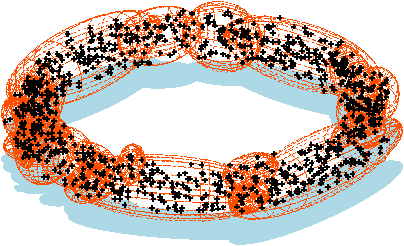
\includegraphics[width=\textwidth]{figures/multinest.pdf}
        \end{block}%
        \vspace{-5pt}
        \begin{block}{\texttt{PolyChord}~\arxiv{1506.00171}}
            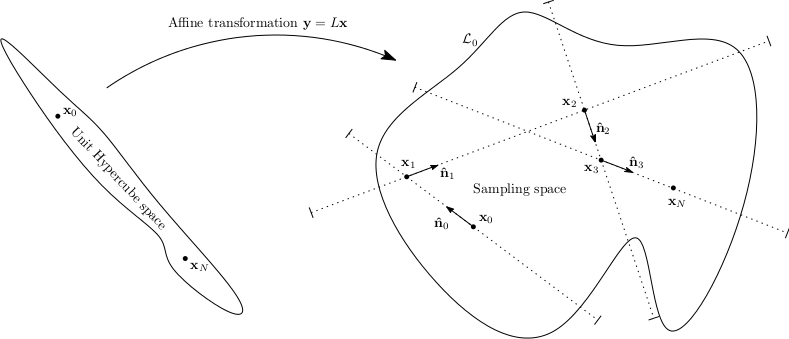
\includegraphics[width=\textwidth]{figures/polychord.png}
        \end{block}



    \end{columns}
\end{frame}

\begin{frame}
    \frametitle{Aside: theoretical work}
    \begin{columns}
        \column{0.5\textwidth}

        This talk will focus on my interdisciplinary work, but I have theoretical interests in:
        \begin{itemize}
            \item Quantum fields in curved spacetime \\\hfill {\small (Mary Letey, Zak Shumaylov, Fruzsina Agocs)}
            \item Poincar\'{e} Gauge Theory \\\hfill {\small (Sinah Legner, Will Barker)}
            \item Future conformal boundary/CPT universes \\\hfill {\small (Metha Prathaban, Wei-Ning Deng)}
            \item Curved finite inflation \hfill {\small (Lukas Hergt)}
        \end{itemize}
        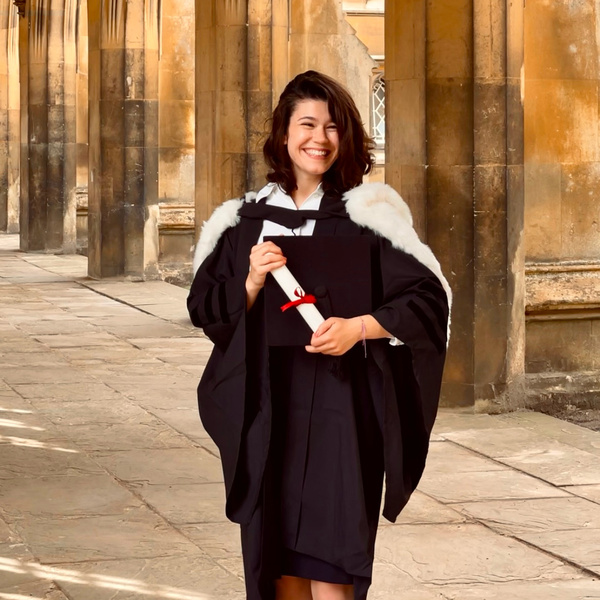
\includegraphics[width=0.125\textwidth]{figures/students/mary_letey.jpg}%
        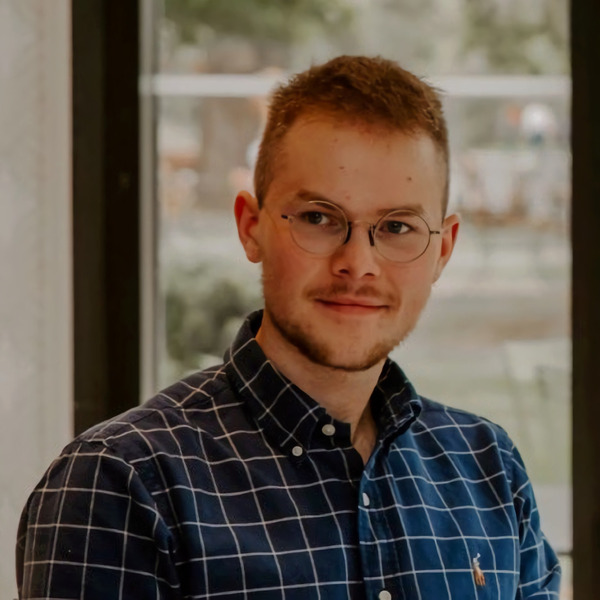
\includegraphics[width=0.125\textwidth]{figures/students/zak_shumaylov.jpg}%
        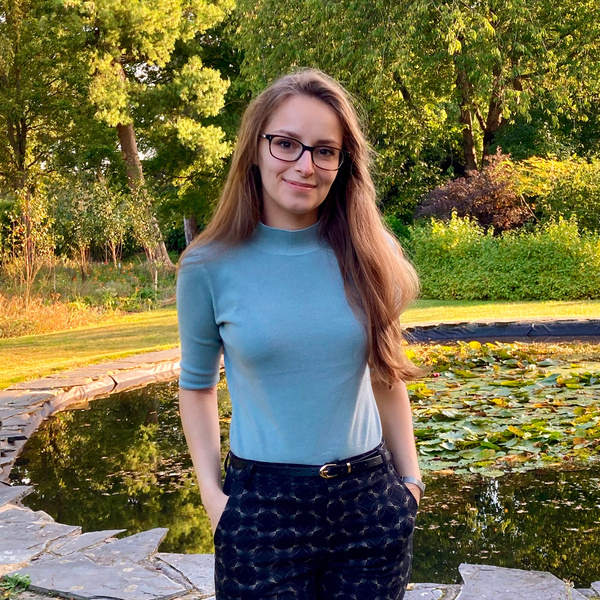
\includegraphics[width=0.125\textwidth]{figures/students/fruzsina_agocs.jpg}%
        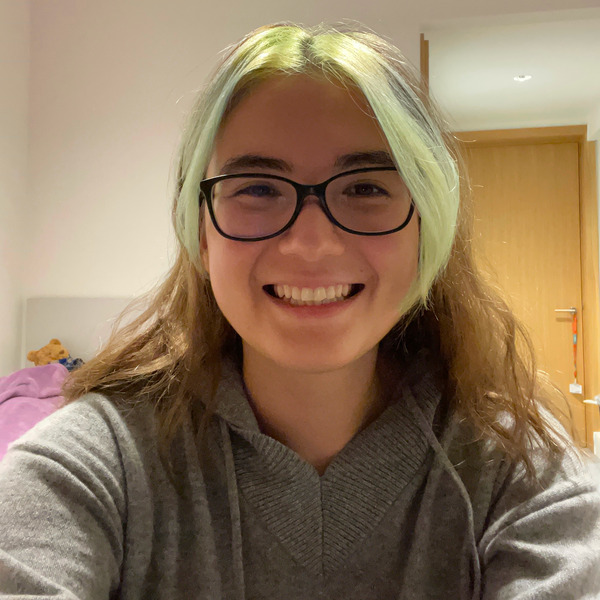
\includegraphics[width=0.125\textwidth]{figures/students/sinah_legner.jpg}%
        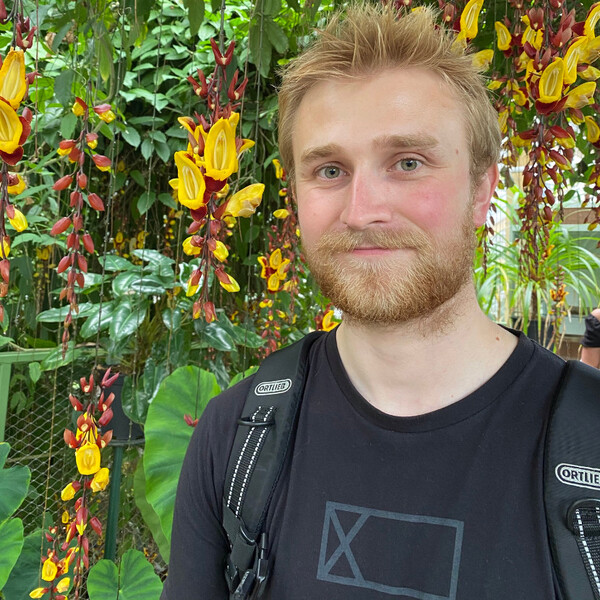
\includegraphics[width=0.125\textwidth]{figures/students/will_barker.jpg}%
        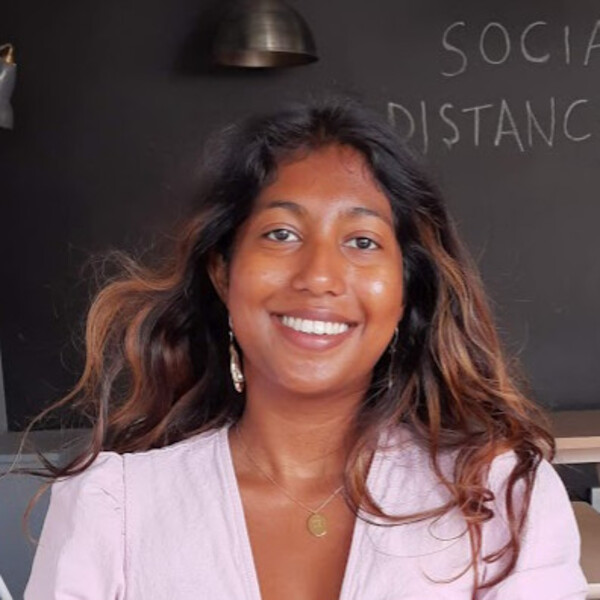
\includegraphics[width=0.125\textwidth]{figures/students/metha_prathaban.jpg}%
        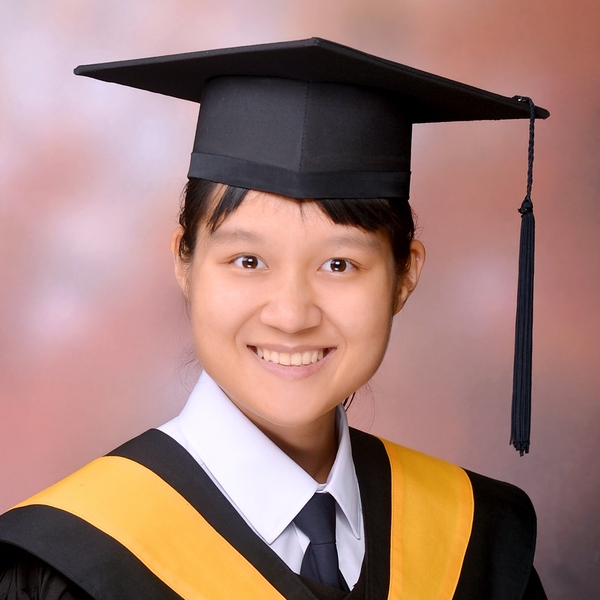
\includegraphics[width=0.125\textwidth]{figures/students/wei-ning_deng.jpg}%
        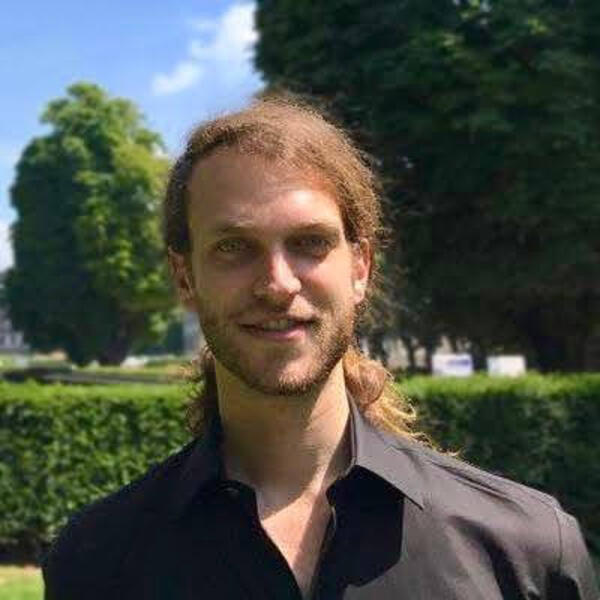
\includegraphics[width=0.125\textwidth]{figures/students/lukas_hergt.jpg}%

        \column{0.5\textwidth}
        \begin{columns}
            \column{0.5\textwidth}
            \begin{overpic}[width=\textwidth]{figures/qic.pdf}
                \put(65,-5) {\tiny \arxiv{1607.04148}}
            \end{overpic}
            \vspace{-5pt}

            \begin{overpic}[width=\textwidth]{figures/pgt.pdf}
                \put(65,-2) {\tiny \arxiv{2003.02690}}
            \end{overpic}
            \column{0.5\textwidth}
            \begin{overpic}[width=\textwidth]{figures/fcb.pdf}
                \put(65,0) {\tiny \arxiv{2111.14588}}
            \end{overpic}

            \begin{overpic}[width=\textwidth]{figures/pps_analytic.pdf}
                \put(65,20) {\tiny \arxiv{1907.08524}}
            \end{overpic}
        \end{columns}
        \vspace{5pt}
        \begin{overpic}[width=\textwidth]{figures/hergt.pdf}
            \put(45,0) {\tiny \arxiv{2211.17248}}
        \end{overpic}
    \end{columns}
\end{frame}

\begin{frame}
    \frametitle{Interdisciplinary work to date}
    \begin{columns}
        \column{0.35\textwidth}
        \begin{itemize}
            \item CMB cosmology
            \item Cosmological tension quantification
            \item \textbf{21cm cosmology}
            \item Radio Instrumentation
            \item \textbf{Gravitational waves}
            \item \textbf{Exoplanets}
            \item \textbf{Particle physics}
            \item Theory of machine learning
            \item Nested sampling theory
            \item Atomistic chemistry
            \item \textbf{Industrial applications}
            \item \ldots
        \end{itemize}
        \column{0.65\textwidth}
        50 minutes is not enough time to cover a decade's publishing.

        \vspace{10pt}

        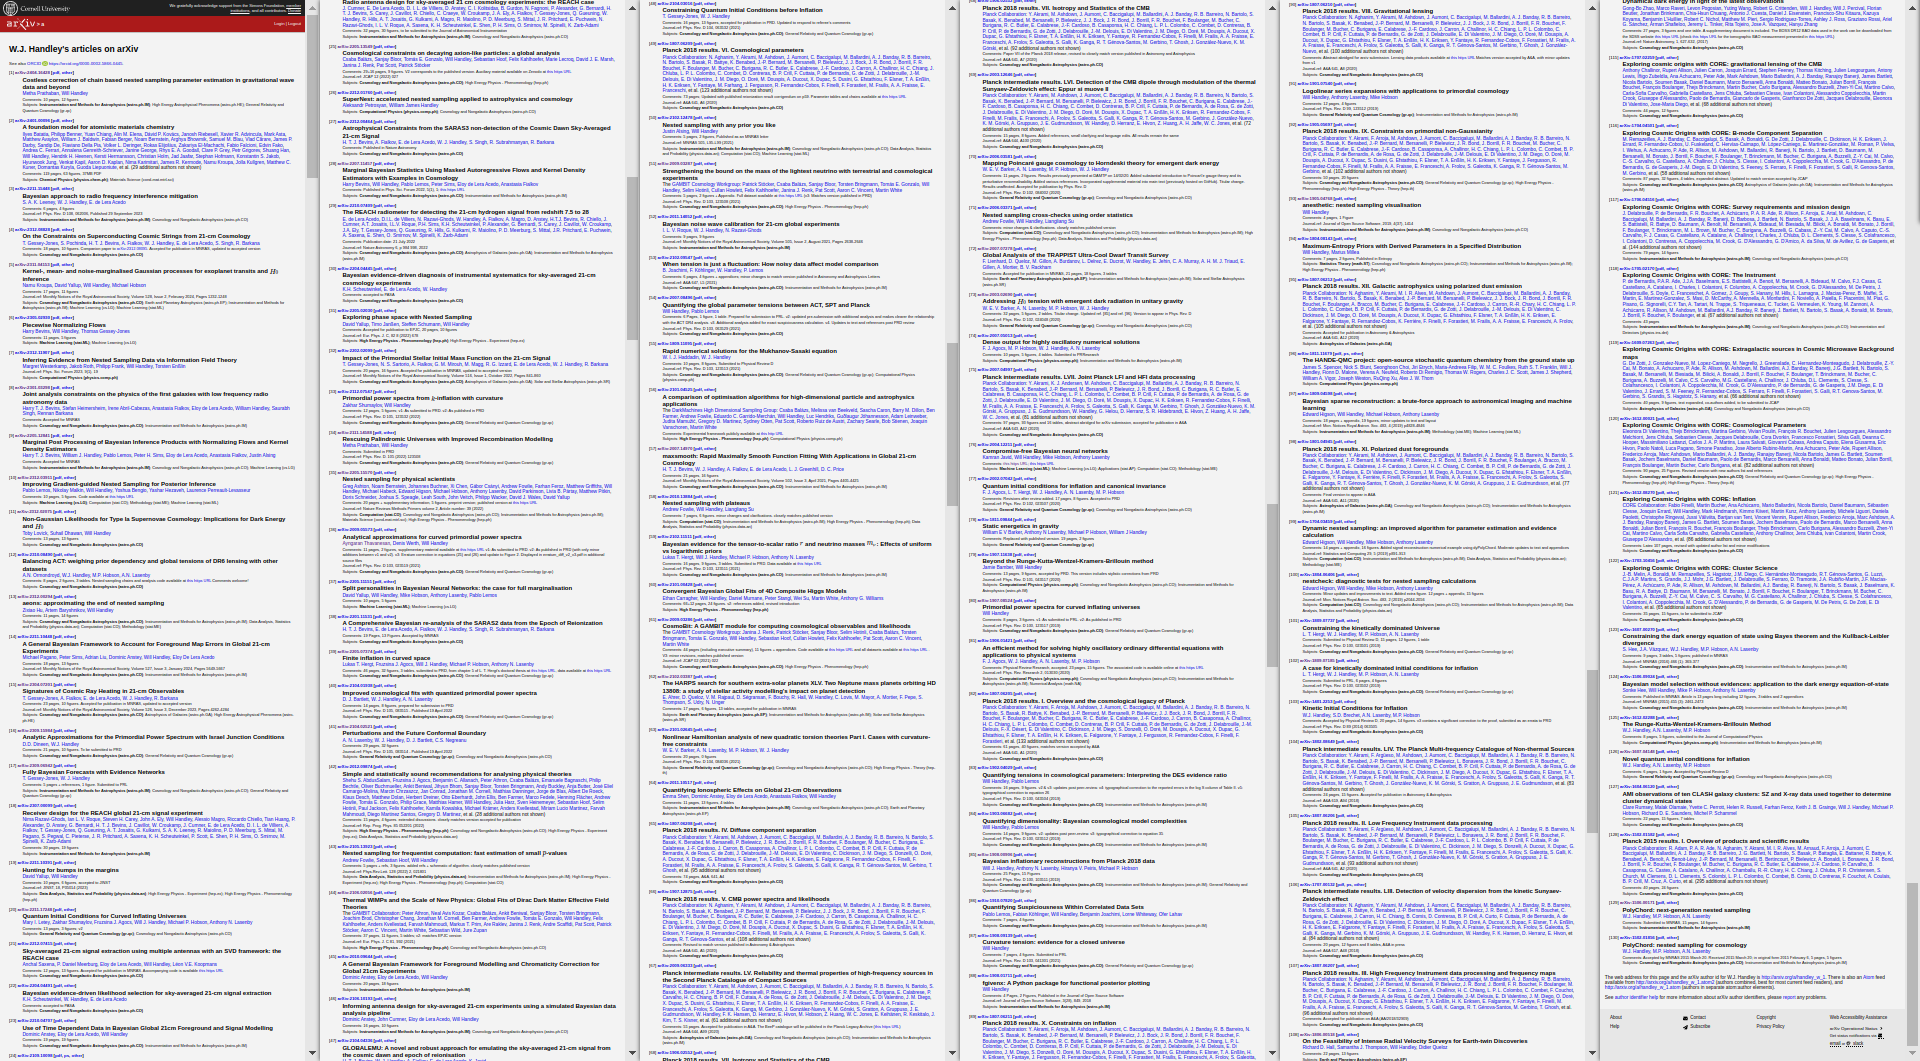
\includegraphics[width=\textwidth]{figures/publishing.png}

        \hfill\textcolor{C0}{\texttt{\href{https://arxiv.org/a/handley_w_1.html}{arxiv.org/a/handley\_w\_1.html}}} 

        Will showcase a targeted subset.
    \end{columns}
\end{frame}

\begin{frame}
    \frametitle{21cm cosmology}
    \student{harry_bevins}{Harry Bevins}{PhD$\to$KICC fellow}

    \begin{columns}
        \column{0.6\textwidth}
        Transferring interdisciplinary ideas into 21cm cosmology with Anastasia Fialkov \& Eloy de Lera Acedo.
        \begin{itemize}
            \item \texttt{maxsmooth} \arxiv{2007.14970}
                \begin{itemize}
                    \item quadratic programming choice arose from quantitative finance consultancy work
                \end{itemize}
            \item \texttt{FlexKnots}
                \begin{itemize}
                    \item importing ideas from inflationary reconstruction into reionisation \arxiv{2310.05608}(Heimersheim) \& ionospheric reconstruction \arxiv{2311.14537}(Shen).
                \end{itemize}
            \item \texttt{margarine} \arxiv{2205.12841} \arxiv{2207.11457}
                \begin{itemize}
                    \item combination of ideas from interdisciplinary fields (emulators, nested sampling, marginal density estimation)
                \end{itemize}
        \end{itemize}
        These techniques are now widely used beyond the Cambridge 21cm community.

        \column{0.4\textwidth}
        \begin{overpic}[height=0.45\textwidth]{figures/maxsmooth_1.pdf}
            \put(0,0) {\tiny \arxiv{2007.14970}}
        \end{overpic}%
        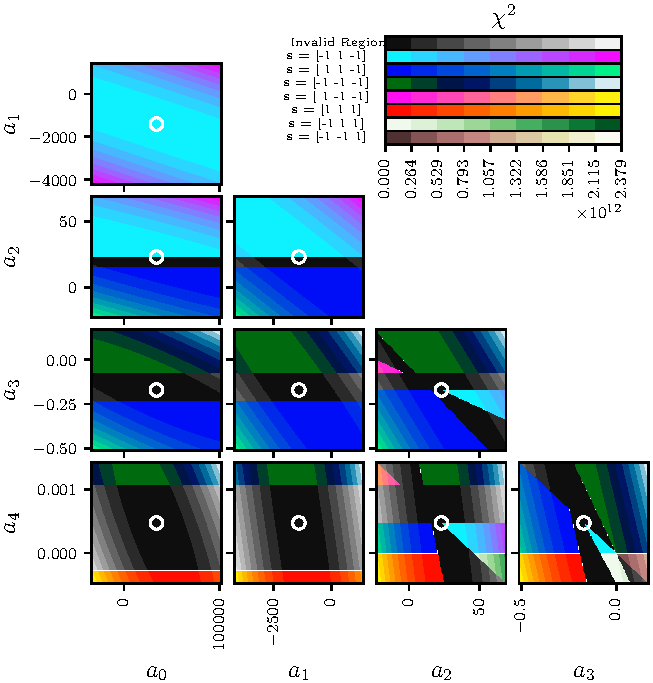
\includegraphics[height=0.45\textwidth]{figures/maxsmooth_2.pdf}
        \vspace{5pt}

        \begin{overpic}[width=\textwidth]{figures/margarine_data.pdf}
            \put(0,0) {\tiny \arxiv{2301.03298}}
        \end{overpic}
    \end{columns}
\end{frame}

\begin{frame}
    \frametitle{REACH: Global 21cm cosmology {\small \arxiv{2210.07409}}}
    \vspace{10pt}
    \begin{columns}
        \column{0.65\textwidth}
        \vspace{-10pt}
        \begin{itemize}
            \item Imaging the universal dark ages using CMB backlight.
            \item $21\text{cm}$ hyperfine line emission from neutral hydrogen.
            \item Global experiments measure monopole across frequency.
            \item Challenge: science hidden in foregrounds $\sim 10^4\times$signal.
            \item Lead data analysis team (REACH first light in January)
            \item Nested sampling woven in from the ground up (calibrator, beam modelling, signal fitting, likelihood selection).
            \item All treated as parameterised model comparison problems.
                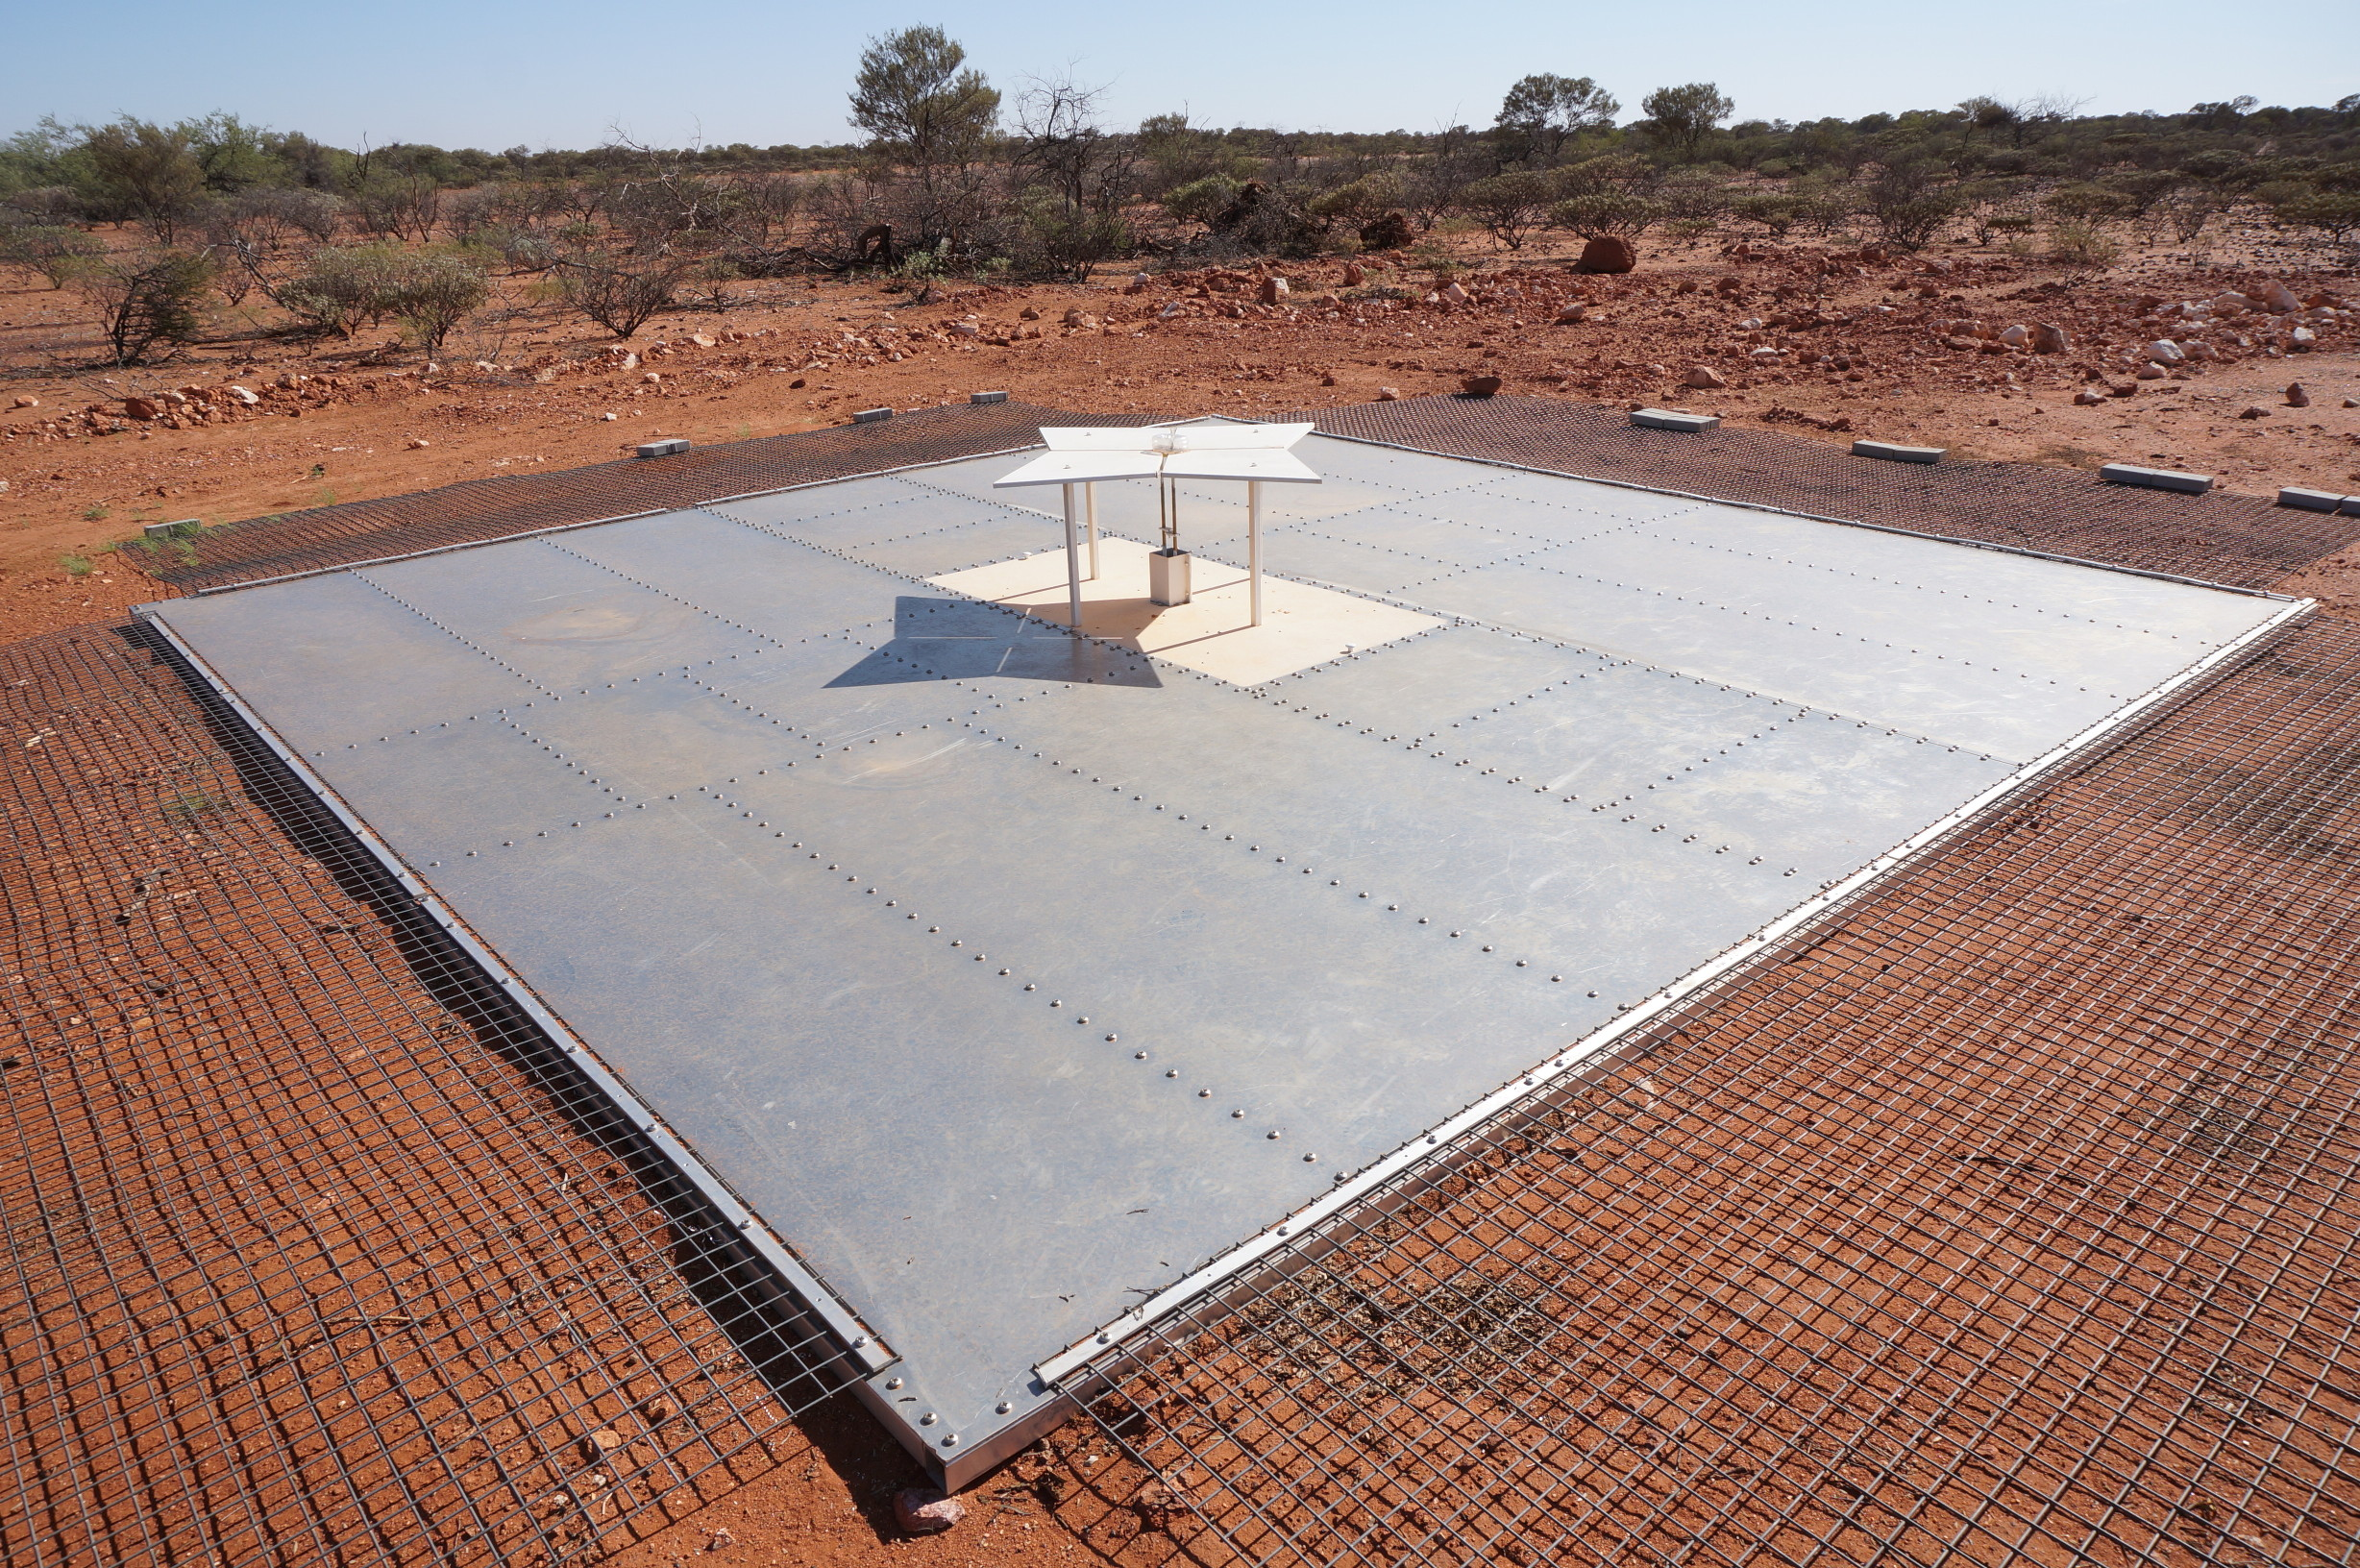
\includegraphics[height=0.3\textwidth]{figures/EDGES_antenna.JPG}
                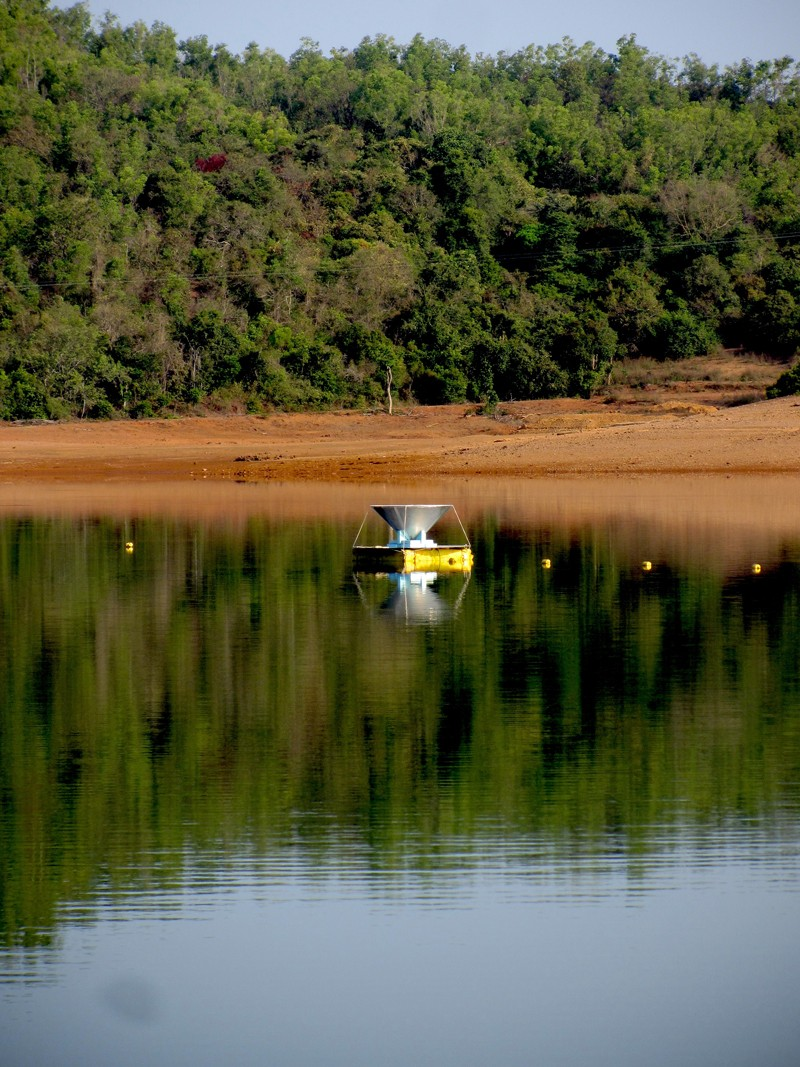
\includegraphics[height=0.3\textwidth]{figures/SARAS.jpg}
                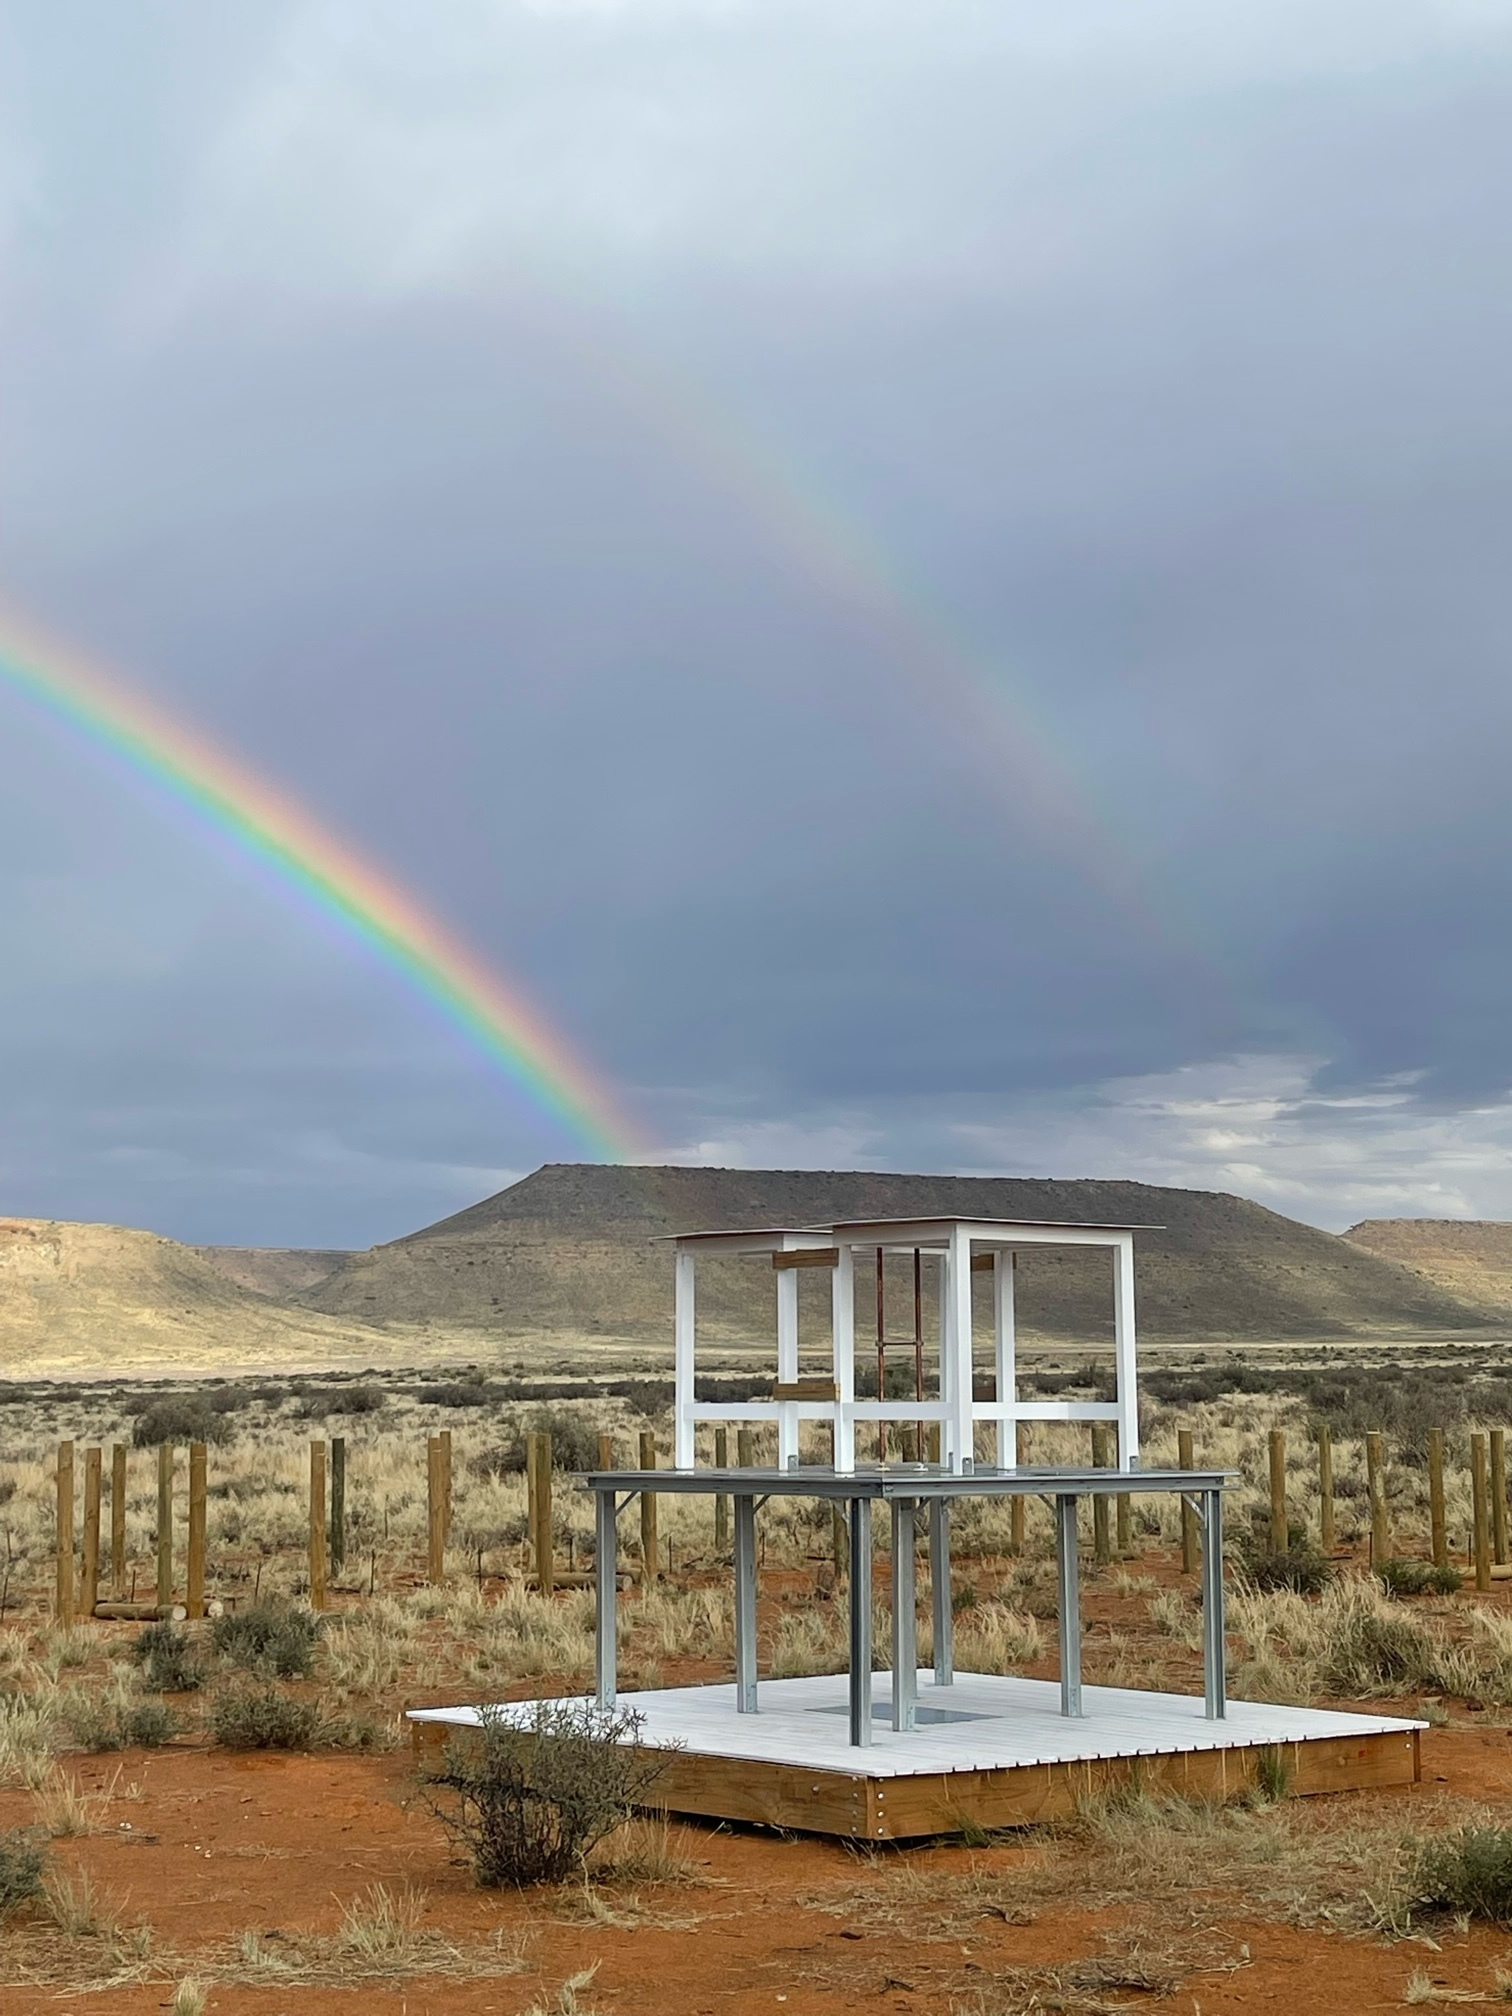
\includegraphics[height=0.3\textwidth]{figures/REACH_2.jpg}
        \end{itemize}
        \column{0.35\textwidth}
        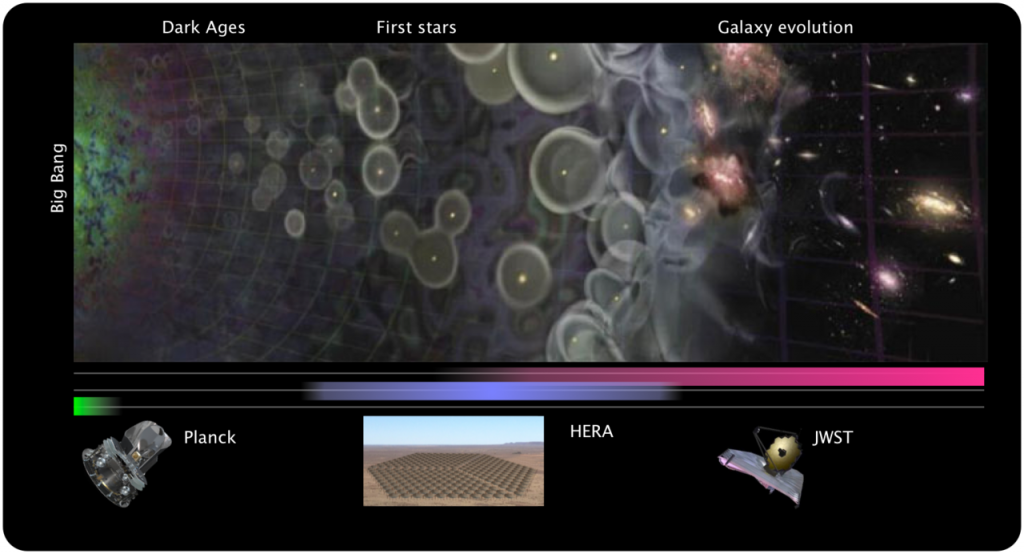
\includegraphics[width=\textwidth]{figures/21cm_1.png}
        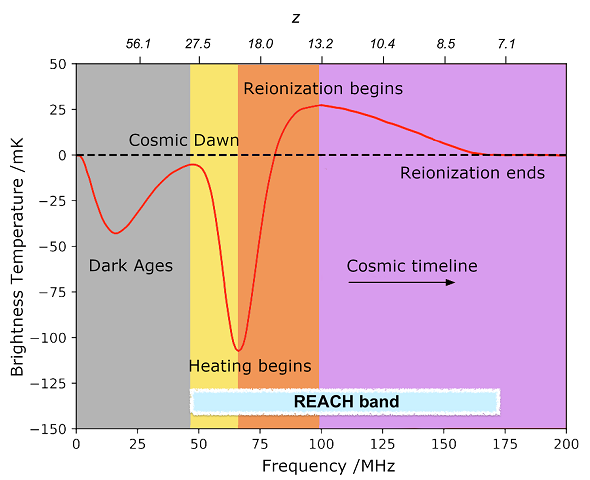
\includegraphics[width=\textwidth]{figures/21cm.png}
    \end{columns}
\end{frame}

\begin{frame}
    \frametitle{Gravitational waves}
    \student{metha_prathaban}{Metha Prathaban}{PhD}
    \begin{columns}
        \column{0.5\textwidth}
        \begin{itemize}
            \item Nested sampling has been used in GW since the beginning [\textcolor{C0}{\href{https://arxiv.org/abs/1602.03840}{GW150914}}]
            \item Work with Alvin Chua \& Chris Moore on transdimensional sampling for EMRI~\arxiv{1803.10210}
            \item Recent work with Metha Prathaban showing new chain-based approaches for improving precision \arxiv{2404.16428}

                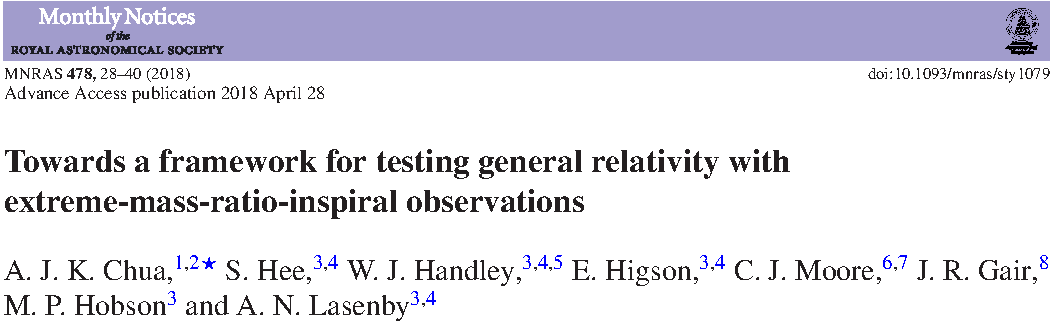
\includegraphics[width=\textwidth]{figures/gw_chua.pdf}

                \vspace{8pt}
                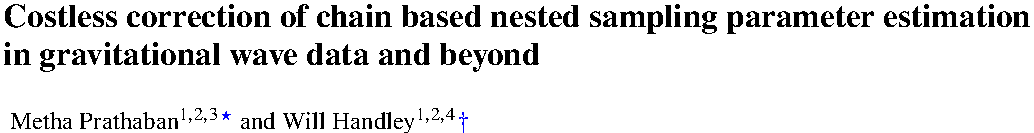
\includegraphics[width=\textwidth]{figures/gw_prathaban.pdf}
        \end{itemize}
        \column{0.5\textwidth}
        \vspace{4pt}

        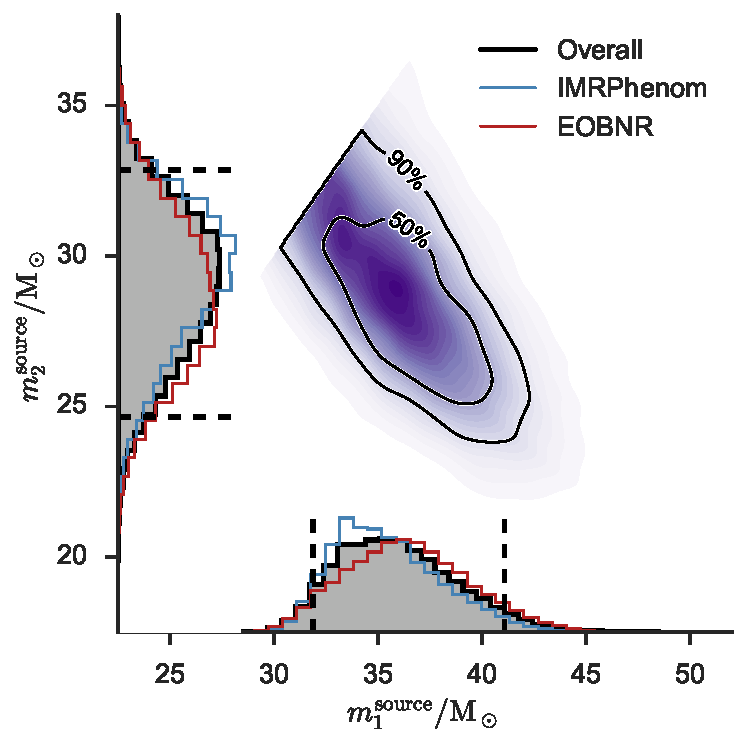
\includegraphics[width=0.49\textwidth]{figures/ligo_m1_m2.pdf}%
        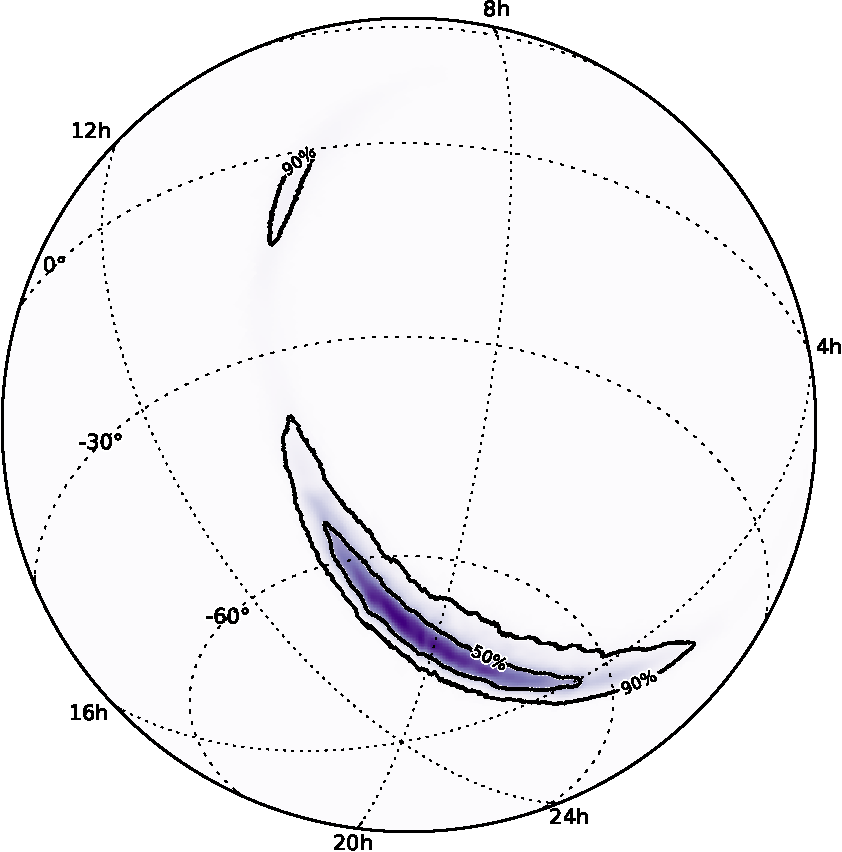
\includegraphics[width=0.49\textwidth]{figures/ligo_lambert-skymap.pdf}
        \vspace{5pt}
        \begin{overpic}[height=0.27\textwidth]{figures/product_space.pdf}%
            \put(12,10) {\tiny \arxiv{1803.10210}}
        \end{overpic}%
        \begin{overpic}[height=0.27\textwidth]{figures/gw_chains.pdf}
            \put(65,-4) {\tiny \arxiv{2404.16428}}
        \end{overpic}
        \begin{itemize}
            \item Discussed use of \texttt{margarine}~\arxiv{2207.11457} as alternative to GW hierarchical modelling at inaugural data science discussion group
        \end{itemize}
    \end{columns}

\end{frame}

\begin{frame}
    \frametitle{Exoplanets}
    \student{namu_kroupa}{Namu Kroupa}{PhD}

    \begin{columns}
        \column{0.5\textwidth}
        \begin{itemize}
            \item Exoplanet science requires solution of subtle inference problems
                \begin{itemize}
                    \item Inference from RV data~\arxiv{1806.00518}
                    \item Survey challenges~\arxiv{2007.07278}
                    \item Stellar activity~\arxiv{2102.03387} 
                \end{itemize}
            \item Gaussian processes+Nested Sampling for transit astronomy~\arxiv{2311.04153}
            \item Potential for further collaboration with Madhu's group who are seeking beyond \texttt{MultiNest} solutions as their problems scale in dimensionality
            \item Ongoing cross-disciplinary theoretical chemistry work may be useful in Paul Rimmer's group.
        \end{itemize}

        \column{0.5\textwidth}
        
\includegraphics[width=\textwidth]{figures/exoplanet_kernel.pdf}%
        \vspace{10pt}
        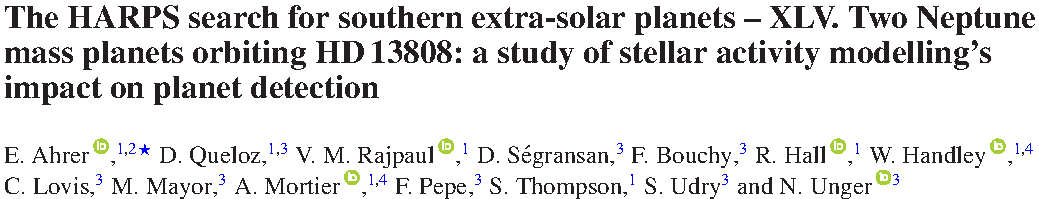
\includegraphics[width=\textwidth]{figures/harps_headline.pdf}%
        \vspace{10pt}
        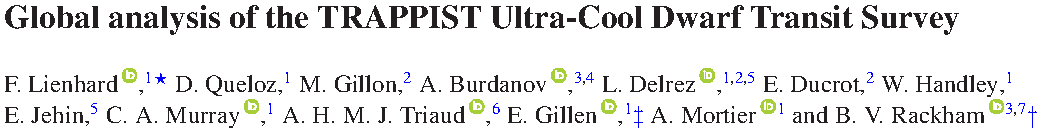
\includegraphics[width=\textwidth]{figures/trappist_headline.pdf}%
        \vspace{10pt}
        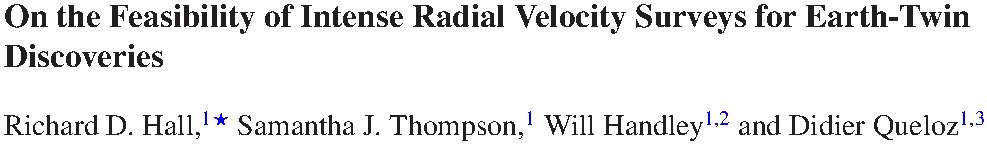
\includegraphics[width=\textwidth]{figures/rv_headline.pdf}%
    \end{columns}
\end{frame}

\begin{frame}
    \frametitle{GAMBIT}
    \framesubtitle{Interdisciplinary case studies}
    \begin{columns}
        \column{0.5\textwidth}
        \begin{itemize}
            \item GAMBIT is an interdisciplinary community and software framework.
            \item Like \texttt{CosmoMC}/\texttt{Cobaya}/\texttt{Bilby}, an organiser of data, likelihoods \& theory, including:
                \begin{itemize}
                    \item Collider data (e.g. LHC)
                    \item Direct detections (e.g. XENON1T)
                    \item Cosmology (\texttt{MontePython})
                    \item Astrophysics (e.g. Bullet Cluster, Supernovae)
                    \item Pulsar timing
                    \item \ldots \& much more
                \end{itemize}
            \item \texttt{GravBit} and \texttt{LowEnergyBit} arising from GAMBIT@KICC workshop
        \end{itemize}
        \column{0.5\textwidth}
        
\includegraphics[height=0.423\textwidth]{figures/students/gambit.png}
        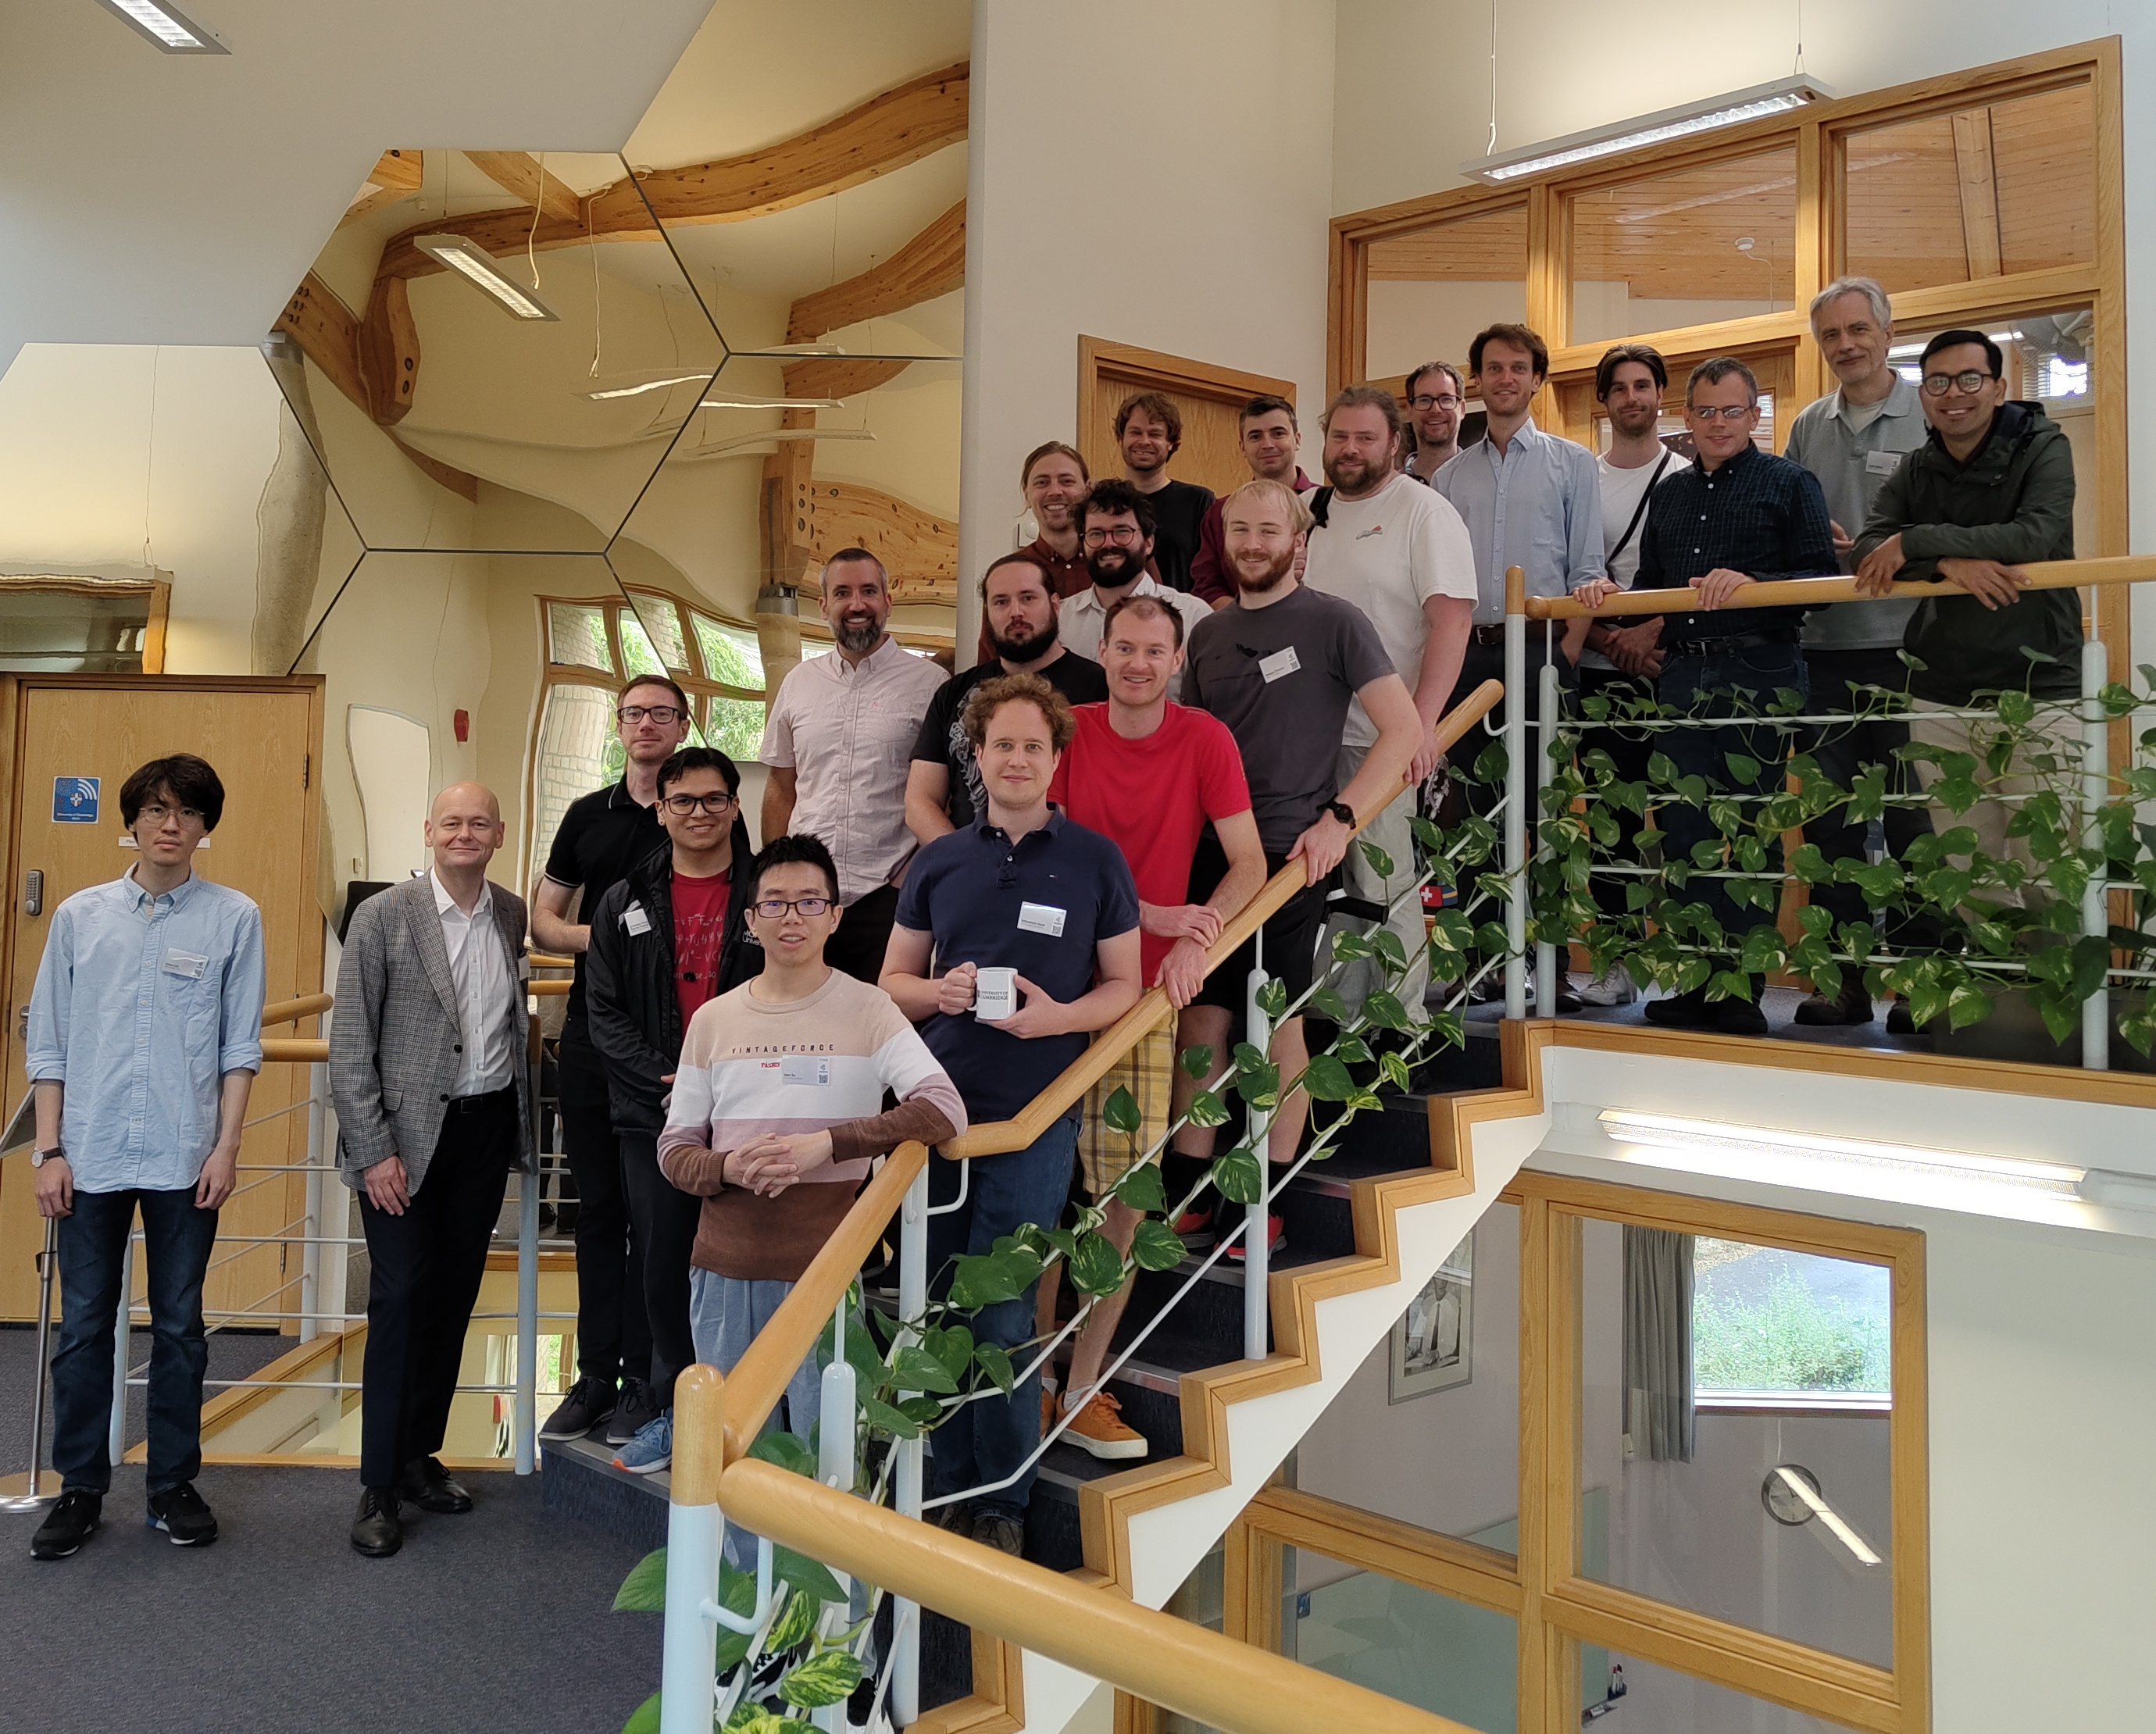
\includegraphics[height=0.423\textwidth]{figures/gambit_kicc.jpg}
        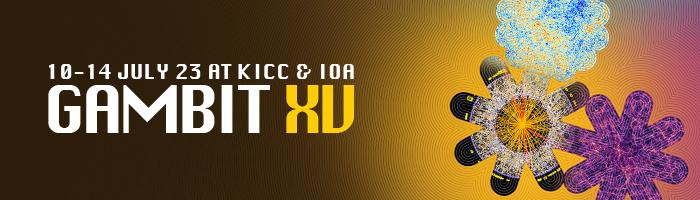
\includegraphics[width=\textwidth]{figures/gambit_meetingbanner.jpg}
    \end{columns}
\end{frame}

\begin{frame}
    \frametitle{GAMBIT: sub-GeV Dark matter constraints}
    \framesubtitle{Interdisciplinary case studies}
    \student{gambit}{Felix Kahlhoefer et al}{GAMBIT cosmo/DM working group}
    \begin{columns}
        \column{0.56\textwidth}
        \begin{itemize}
            \item Physical model of sub-GeV thermal dark matter with a dark photon mediator~$A$:
        \end{itemize}
        \vspace{-10pt}
        \begin{align*}
            \small
            \mathcal{L}_\text{int} =& -\frac{1}{2} m_{A'}^2 A'^\mu A'_\mu - \frac{1}{4} A'^{\mu\nu}A'_{\mu\nu} -\kappa e A'^\mu \sum_{f} q_f \overline{f} \gamma_\mu f \,,
            \normalsize
        \end{align*}
        \vspace{-15pt}
        \begin{itemize}
            \item Constrain using cosmological, astrophysical, accelerator \& direct detection data.
            \item Bayesian Model comparison of Fermion~$\psi$ vs scalar~$\Phi$ models (scalar preferred).
        \end{itemize}
        \vspace{-10pt}
        \begin{align*}
            \small
            \mathcal{L}_\psi  =& \bar{\psi}(i \slashed{\partial} - m_\text{DM}) \psi + g_\text{DM} A'^\mu \bar{\psi} \gamma_\mu \psi \,,\\
            \mathcal{L}_\Phi  =& |\partial_\mu \Phi|^2 - m_\text{DM}^2 |\Phi|^2 - g_\text{DM}^2 A'_\mu A'^\mu |\Phi|^2 \\ &+ i g_\text{DM} A'^\mu \left[\Phi^\ast (\partial_\mu \Phi) - (\partial_\mu \Phi^\ast) \Phi\right]\,,
            \normalsize
        \end{align*}
        \column{0.44\textwidth}
        \vspace{10pt}
        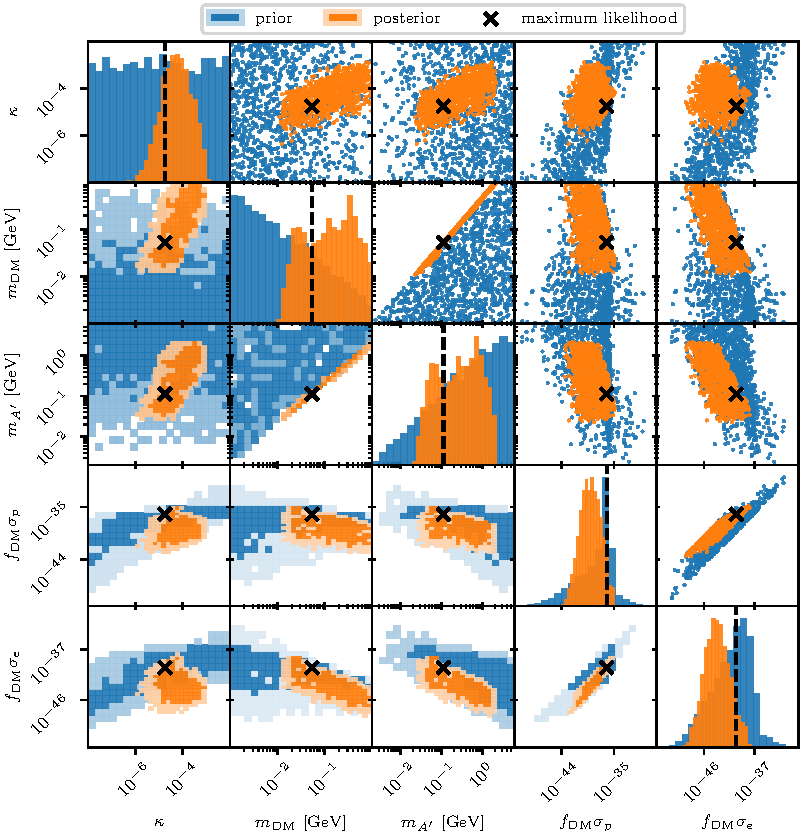
\includegraphics[width=\textwidth]{figures/Bayes_SubGeVDM_fermion_RDprior_allDM_asym_observables.pdf}
    \end{columns}
\end{frame}

\begin{frame}
    \frametitle{PolyChord Ltd: interdisciplinary R\&D spinout}
    \framesubtitle{Interdisciplinary case studies}
    \only<1-4>{
        \student{watkinson-headshot}{Catherine Watkinson}{Senior Data Scientist}
    }
    \only<5->{
        \student{mcaloone-headshot}{Thomas Mcaloone}{PhD $\to$ Data Scientist}
    }
    \begin{columns}
        \column{0.6\textwidth}
        \begin{itemize}
            \item Techniques have been spun-out (PolyChord Ltd) to:
            \item Protein folding
                \begin{itemize}
                    \item Navigating free energy surface.
                    \item Computing misfolds.
                    \item Thermal motion.
                \end{itemize}
            \item Nuclear fusion reactor optimisation
                \begin{itemize}
                    \item multi-objective.
                    \item uncertainty propagation.
                \end{itemize}
            \item Telecoms \& DSTL research (MIDAS)
                \begin{itemize}
                    \item Optimising placement of transmitters/sensors.
                    \item Maximum information data acquisition strategies.
                \end{itemize}
        \end{itemize}
        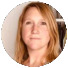
\includegraphics[width=0.08\textwidth]{figures/headshots/catherine-watkinson-polychord.jpg}%
        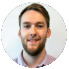
\includegraphics[width=0.08\textwidth]{figures/headshots/thomas-macaloone-polychord.jpg}%
        
\includegraphics[width=0.08\textwidth]{figures/headshots/angus-peters-polychord.jpg}%
        
\includegraphics[width=0.08\textwidth]{figures/headshots/tamas-stenzel-polychord.jpg}%
        
\includegraphics[width=0.08\textwidth]{figures/headshots/david-yallup-polychord.jpg}%
        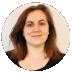
\includegraphics[width=0.08\textwidth]{figures/headshots/rebecca-handley-polychord.jpg}%
        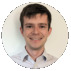
\includegraphics[width=0.08\textwidth]{figures/headshots/adam-ormondroyd-polychord.jpg}%
        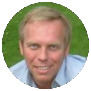
\includegraphics[width=0.08\textwidth]{figures/headshots/mike-hobson-polychord.jpg}%
        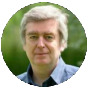
\includegraphics[width=0.08\textwidth]{figures/headshots/anthony-lasenby-polychord.jpg}%
        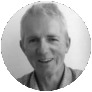
\includegraphics[width=0.08\textwidth]{figures/headshots/mike-handley-polychord.jpg}%
        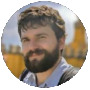
\includegraphics[width=0.08\textwidth]{figures/headshots/will-handley-polychord.jpg}%
        \column{0.4\textwidth}
        \includegraphics<1|handout:0>[width=\textwidth]{figures/protein_1.png}%
        \includegraphics<2          >[width=\textwidth]{figures/protein_2.png}%
        \includegraphics<3|handout:0>[width=\textwidth]{figures/protein_3.png}%
        \includegraphics<4|handout:0>[width=\textwidth]{figures/lcoe.png}%
        %\includegraphics<5|handout:0>[width=\textwidth]{figures/tdoa-cropped-1-crop.pdf}%
        %\includegraphics<6|handout:0>[width=\textwidth]{figures/tdoa-cropped-2-crop.pdf}%
        %\includegraphics<7|handout:0>[width=\textwidth]{figures/tdoa-cropped-3-crop.pdf}%
        \includegraphics<5|handout:0>[width=\textwidth]{figures/DKL_contour-cropped-crop.pdf}%
        \includegraphics<6|handout:0>[width=\textwidth]{figures/mean_DKL_optimise-3-crop.pdf}%
        \includegraphics<7|handout:0>[width=\textwidth]{figures/mean_DKL_optimise-4-crop.pdf}%
        \includegraphics<8|handout:0>[width=\textwidth]{figures/mean_DKL_optimise-5-crop.pdf}%
    \end{columns}
\end{frame}

\begin{frame}
    \frametitle{DSTL: Bayesian OODA loops}
    \framesubtitle{Interdisciplinary case studies}
    \begin{columns}
        \column{0.5\textwidth}
        \begin{itemize}
            \item Work through Isaac Newton Institute with Defence Science \& Technology Laboratory.
            \item Quantification of ``OODA'' loop concept from litigation, business, law enforcement, management and military strategy
        \end{itemize}


        \begin{columns}
            \column{0.5\textwidth}
            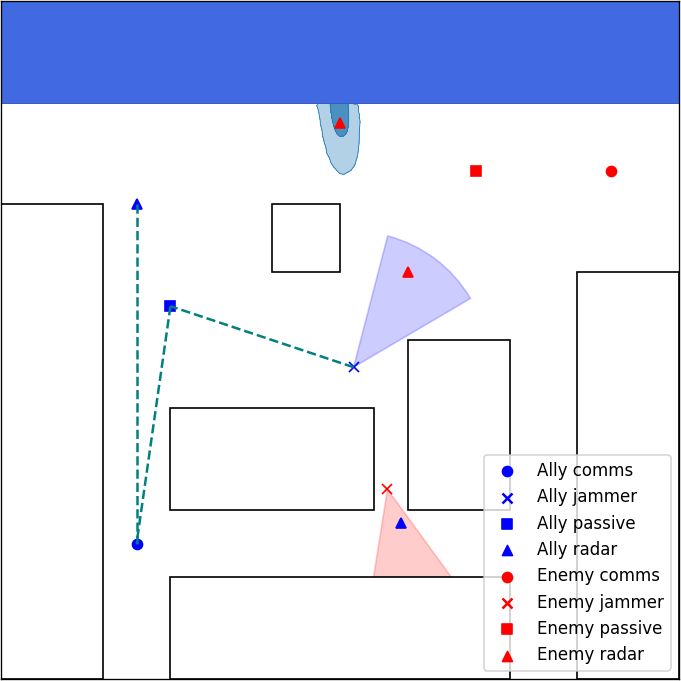
\includegraphics[width=\textwidth]{figures/midas.png}%
            \column{0.5\textwidth}
            \begin{itemize}
                \item Two-way research interaction between government and academia.
                \item techniques now being used in REACH antenna design~\arxiv{2309.06942}
            \end{itemize}
        \end{columns}


        \column{0.5\textwidth}
        \begin{minipage}[]{0.6\textwidth}
            \begin{tikzpicture}[
                    node distance=5mm,
                    >=stealth, auto,
                    every state/.style={
                        rectangle, rounded corners, minimum height=6em, minimum width=2em,
                        text width=3cm, align=center
                    }
                ]


                \node[state, fill=C3!20] (q14) {{\textbf{Act}}
                    \\ 
                    \small
                    Execute strategy $\bm{s}$\\
                    Replace prior $\pi$ with posterior $\mathcal{P}$
                };
                \node[state, fill=C0!20] (q12) [above=of q14] { {\textbf{Observe}} 
                    \\
                    \small
                    Collect data $\bm{D}$ about system $\bm{\theta}$ using strategy $\bm{s}$.
                };
                \node[state, fill=C1!20] (q23) [right=of q12] { {\textbf{Orient}} 
                    \\
                    \small
                    Update knowledge from prior~$\pi(\bm{\theta})$ to posterior~$\mathcal{P}(\bm{\theta}|\bm{D})$.
                };
                \node[state, fill=C2!20] (q34) [below=of q23] { {\textbf{Decide}} 
                    \\
                    \small
                    choose strategy $\bm{s}$ using information $\hat{\mathcal{D}}_\mathrm{KL}(\bm{s}|\mathcal{P})$.
                };
                \begin{scope}[bend left]%
                    \path[thick,-{Latex[width=2mm]}]   (q14.north) edge node {} (q12.south)
                    (q12.east) edge node {} (q23.west)
                    (q23.south) edge node {} (q34.north)
                    (q34.west) edge node {} (q14.east);
                \end{scope}

                \node[align=center] (e) at (barycentric cs:q12=1,q23=1,q34=1,q14=1) {\Large\textbf{MIDAS}};

            \end{tikzpicture}
        \end{minipage}%
    \end{columns}
\end{frame}

\begin{frame}
    \frametitle{Beginning the golden age of astronomy data}
    \begin{columns}
        \column{0.47\textwidth}
        \begin{itemize}
            \item Over our research lifetimes we will see next-generation data rates across the electromagnetic spectrum \& beyond:
                \begin{description}
                    \item[Radio] SKA \textit{et al}
                    \item[Micro] SO/CMB-S4/LiteBIRD
                    \item[IR] JWST, Roman
                    \item[Optical] Euclid, DESI, Rubin, EELT
                    \item[X-ray] Athena
                    \item[Gamma-ray] e-ASTROGAM
                    \item[Gravitational] LIGO/LVK$^+$/LISA
                    \item[Particle] CTA, IceCube, KM3NeT
                \end{description}
        \end{itemize}
        \column{0.55\textwidth}

        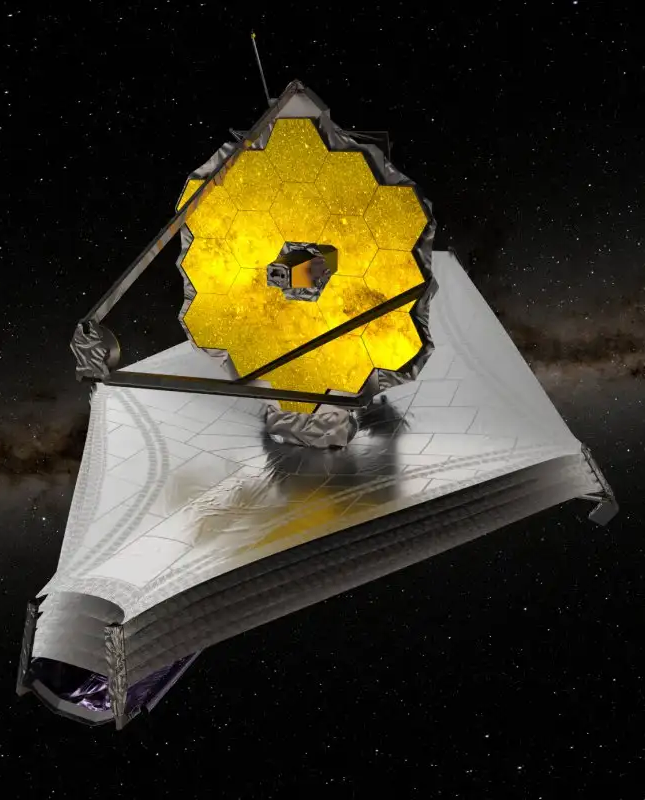
\includegraphics[height=0.145\textwidth]{figures/telescopes/jwst.png}%
        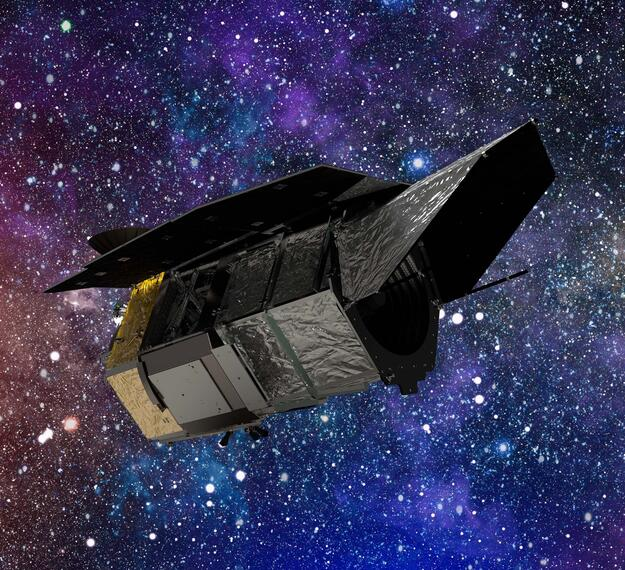
\includegraphics[height=0.145\textwidth]{figures/telescopes/roman.jpg}%
        \includegraphics[height=0.145\textwidth]{figures/telescopes/euclid.jpeg}%
        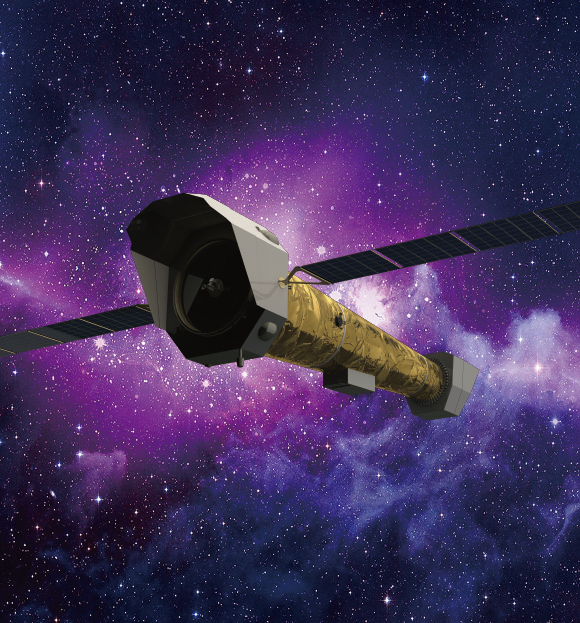
\includegraphics[height=0.145\textwidth]{figures/telescopes/athena.jpg}%
        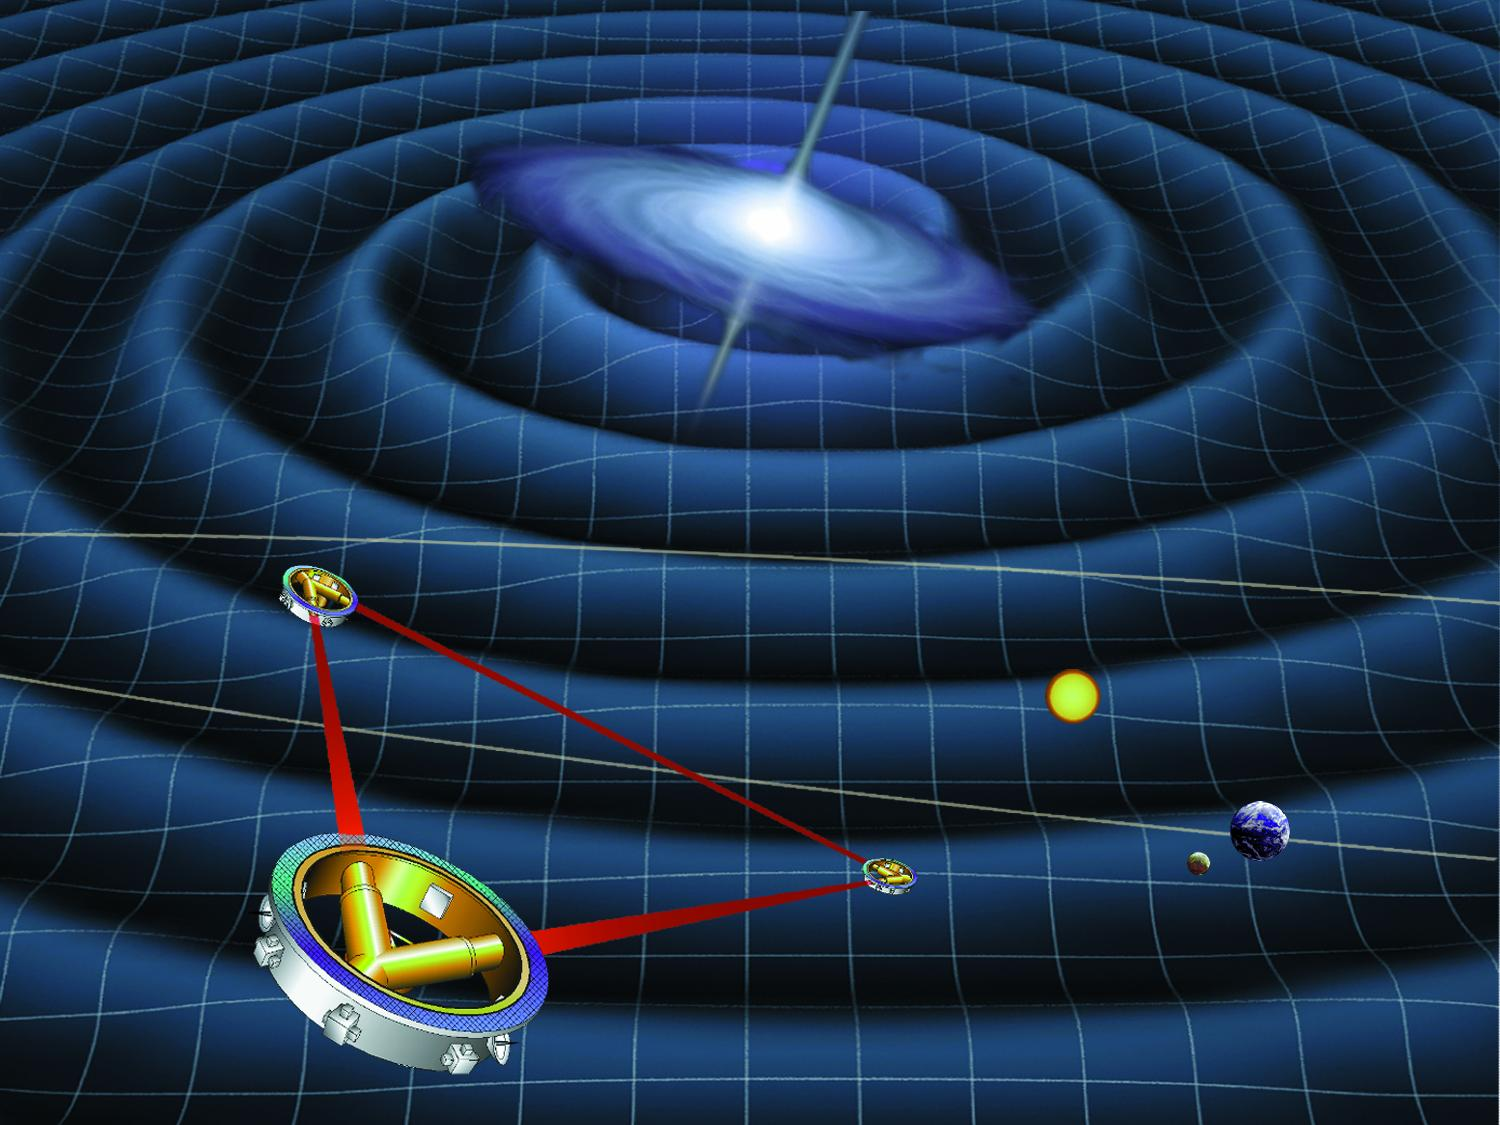
\includegraphics[height=0.145\textwidth]{figures/telescopes/lisa.jpg}%
        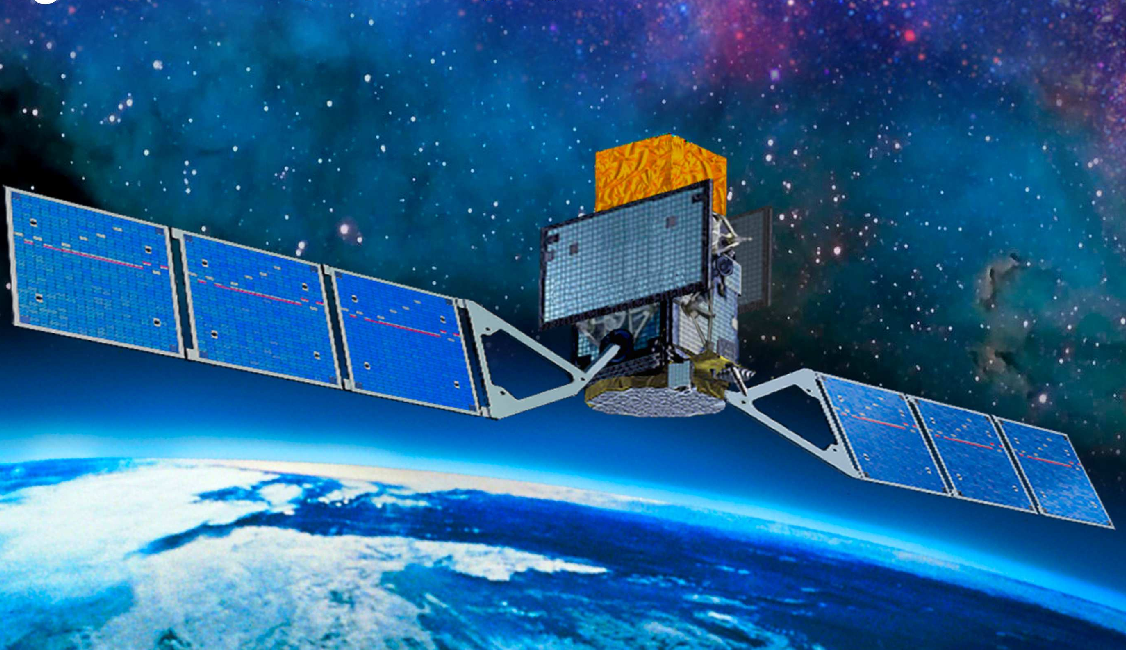
\includegraphics[height=0.145\textwidth]{figures/telescopes/e-ASTROGAM.pdf}%
        \vspace{-1pt}

        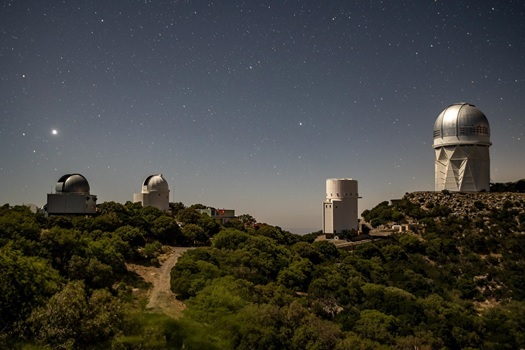
\includegraphics[height=0.15183\textwidth]{figures/telescopes/desi.jpg}%
        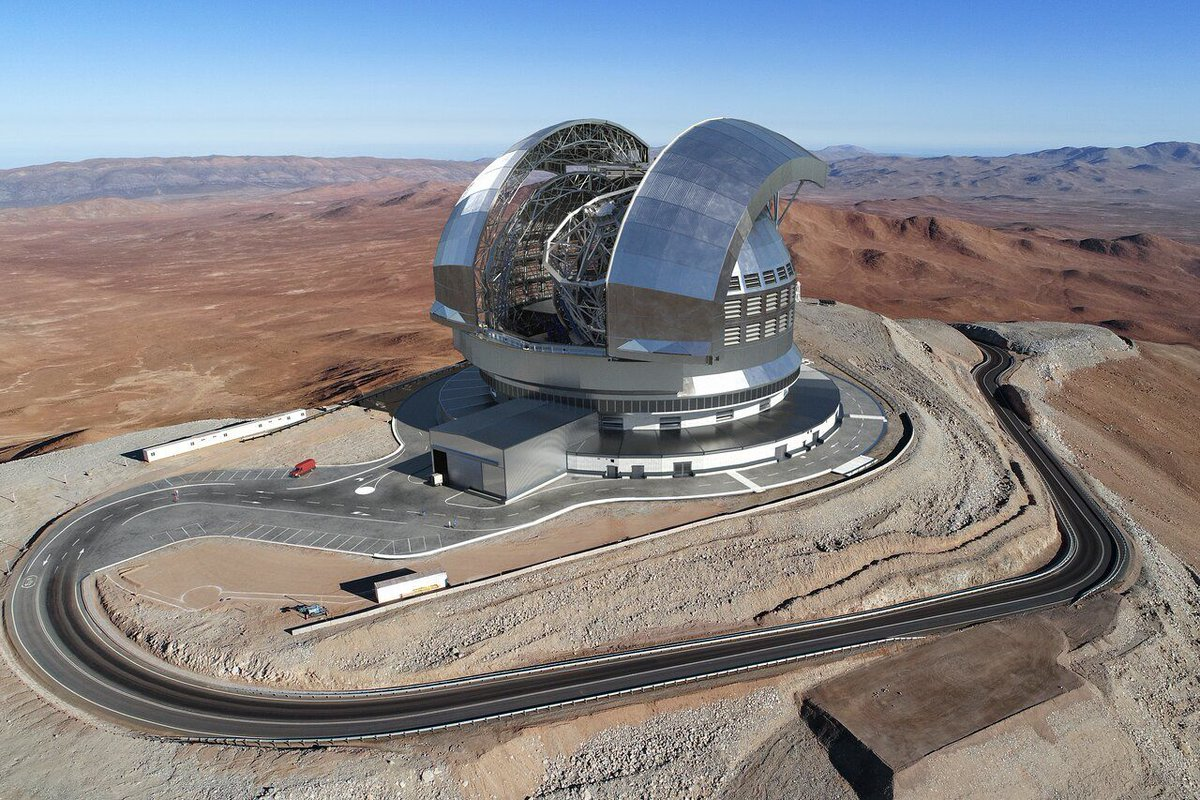
\includegraphics[height=0.15183\textwidth]{figures/telescopes/eelt.jpg}%
        \includegraphics[height=0.15183\textwidth]{figures/telescopes/ska.jpg}%
        \includegraphics[height=0.15183\textwidth]{figures/telescopes/SO.jpg}%
        \vspace{-1pt}

        \includegraphics[height=0.18428\textwidth]{figures/telescopes/ligo.jpg}%
        \includegraphics[height=0.18428\textwidth]{figures/telescopes/km3n.jpg}%
        \includegraphics[height=0.18428\textwidth]{figures/telescopes/icecube.jpg}%
        \includegraphics[height=0.18428\textwidth]{figures/telescopes/CTA.jpg}%

        \begin{itemize}
            \item This ever-increasing statistical weight will mean true accuracy demands rigorous attention to systematics.
            \item This applies to all of cosmology, astrophysics, particle physics and beyond.
        \end{itemize}

    \end{columns}
\end{frame}

\begin{frame}
    \frametitle{Tensions in cosmology}
    \begin{columns}
        \column{0.38\textwidth}
        \begin{block}{Hubble}
            \begin{overpic}[width=\textwidth]{figures/hubble_tension.pdf}
                \put(72,37) {\tiny \arxiv{1907.05922}}
            \end{overpic}
        \end{block}
        \column{0.17\textwidth}
        \begin{block}{Weak lensing}
            \begin{overpic}[width=\textwidth]{figures/kids_tension.pdf}
                \put(13,18) {\tiny \arxiv{2007.15632}}
            \end{overpic}%
        \end{block}
        \column{0.36\textwidth}
        \begin{block}{\hfill other $w_0$/$\Omega_K$/$\nu$?}
            \begin{overpic}[width=0.48\textwidth]{figures/desi_tension.pdf}
                \put(0,90) {\tiny \arxiv{2404.03002}}
            \end{overpic}%
            \begin{overpic}[width=0.48\textwidth]{figures/curvature_3.pdf}
                \put(54,20) {\tiny \arxiv{1908.09139}}
            \end{overpic}%
        \end{block}
    \end{columns}

    \begin{columns}
        \column{0.75\textwidth}
        \begin{itemize}
            \item Tensions have been appearing in cosmology over the last five years.
            \item Though their significance may be debatable, they have revealed a gap in the armour of modern data analysis.
            \item Likelihood-based methods have to assume a fiducial cosmology. 
            \item This will cast greater doubt on the robustness of our conclusions from stage 4 surveys and beyond.
        \end{itemize}
        \column{0.25\textwidth}
        \begin{block}{\tiny DESI BAO paper: \arxiv{2404.03000}}
            \includegraphics[width=\textwidth]{figures/desi_fiducial.pdf}
        \end{block}
    \end{columns}

\end{frame}

\begin{frame}
    \frametitle{The real tensions in the room}


    \begin{columns}
        \column{0.34\textwidth}
        \begin{block}{Dark tension}
            \includegraphics[width=\textwidth]{figures/pie_chart.jpg}
        \end{block}
        \column{0.26\textwidth}
        \begin{block}{Initial conditions}
            \includegraphics[width=\textwidth]{figures/multiverse.jpg}
        \end{block}
        \column{0.32\textwidth}
        \begin{block}{Quantum gravity}
            \includegraphics[width=\textwidth]{figures/quantum_gravity.jpeg}
        \end{block}
    \end{columns}
    \begin{columns}
        \column{0.6\textwidth}
        \begin{itemize}
            \item These are existential questions that don't go away if $\Lambda$CDM is phenomenologically correct\ldots
            \item \ldots and if it is, we will need an interdisciplinary approach that goes far beyond cosmology (using astronomy, collider \& experimental physics).
        \end{itemize}
        \column{0.4\textwidth}
        \begin{itemize}
            \item The GW redshift frontier, time domain astronomy \& 21cm SKA will be the key tools for challenging our astronomical understanding.
        \end{itemize}
    \end{columns}
\end{frame}

\begin{frame}
    \frametitle{The future: simulation-based inference}
    \student{kilian_scheutwinkel}{Kilian Scheutwinkel}{PhD}
    \vspace{5pt}
    \begin{itemize}
        \item Traditional Likelihood-based inference (LBI) requires knowledge of the likelihood $P(D|\theta)$
            \begin{itemize}
                \item For the CMB, it is possible to compute Probability(Sky$|\Lambda$CDM) [with caveats]
                \item For almost everybody else (different models, more evolved systems), the likelihood is approximate
            \end{itemize}
        \item Simulation-based inference learns the likelihood from physical simulations $\theta\to D$.
    \end{itemize}
    \begin{columns}
        \column{0.65\textwidth}
        \begin{itemize}
            \item Can extract nonlinear information from data.
            \item Do not need to assume a fiducial model, since data covariance is implicit in simulations.
            \item Users do not need to know advanced statistics
                \begin{itemize}
                    \item For this reason alone, it will come to dominate the next generation $\Rightarrow$ imperative to build a principled understanding!
                \end{itemize}
            %\item The current state of the art is achieved with \textit{Neural}~estimation
            \item My interest has been in understanding how essential machine learning is by building analytics \tthref{github.com/handley-lab/lsbi}
            \item Have also made progress on the first simulation-based nested sampler \texttt{PolySwyft} (presenting at EuCAIFCon)
        \end{itemize}
        \column{0.35\textwidth}
        \begin{overpic}[width=\textwidth]{figures/des_sbi.pdf}
            \put(65,80) {\tiny \arxiv{2403.02314}}
            \put(65,73) {\tiny (Jeffrey et DES)}
        \end{overpic}
    \end{columns}
\end{frame}

\begin{frame}
    \frametitle{ERC grant: COSMOTENSION \hspace{95pt}\small \tthref{willhandley.co.uk/ERC.pdf}}
    \framesubtitle{Resolving cosmological tensions with diverse data, novel theories and Bayesian machine learning}

    \begin{columns}
        \column{0.6\textwidth}
        \begin{itemize}
            \item ERC starting grant $\Rightarrow$ UKRI Frontier, commencing October 2024.
            \item Funds 3 PDRAs and 4 PhDs over 5 years.
            \item Research programme centered around combining novel theories of gravity, Boltzmann solvers~\arxiv{1906.01421}, reconstruction~\arxiv{1908.00906}, nested sampling \& simulation-based inference (n\'{e}e LFI).
            \item Aims to disentangle cosmological tensions $H_0$, $\sigma_8$, $\Omega_K$ with next-generation data analysis techniques.
        \end{itemize}
        \column{0.4\textwidth}
        \includegraphics[width=\textwidth]{figures/denseoutput.pdf}
        \includegraphics[width=\textwidth]{figures/pps.pdf}
        \includegraphics[width=\textwidth]{figures/gantt.pdf}
    \end{columns}

\end{frame}

\begin{frame}
    \frametitle{Conclusions}
    \framesubtitle{\tthref{github.com/handley-lab}}
    \begin{columns}
        \column{0.6\textwidth}
        \begin{itemize}
            \item The astronomy challenges of our generation are interdisciplinary.
            \item Interdisciplinary approaches are two-way streets for innovation.
            \item Simulation-based inference represents the frontier of how we will all be doing data analysis.
            \item Our research programme at the interface between theory, observation and inference is well-placed to explore the interdisciplinary frontier.
        \end{itemize}

        \column{0.4\textwidth}
        \includegraphics[height=0.32\textwidth]{logos/ukri}\hfill
        \includegraphics[height=0.32\textwidth]{logos/ukerc}\hfill
        \includegraphics[height=0.32\textwidth]{logos/royalsociety}

        \centerline{
            \includegraphics[width=0.8\textwidth]{logos/dirac.png}%
        }
    \end{columns}
    \vspace{10pt}


    \tikz[overlay,remember picture]
    \node[anchor=north east] (A) at ($(current page.north east)+(0,0)$) {
        \includegraphics[width=0.09\textheight]{figures/students/adam_ormondroyd.jpg}%
        \includegraphics[width=0.09\textheight]{figures/students/david_yallup.jpg}%
        \includegraphics[width=0.09\textheight]{figures/students/dily_ong.jpg}%
        \includegraphics[width=0.09\textheight]{figures/students/felicity_ibrahim.jpg}%
        \includegraphics[width=0.09\textheight]{figures/students/george_carter.jpg}%
        \includegraphics[width=0.09\textheight]{figures/students/harry_bevins.jpg}%
        \includegraphics[width=0.09\textheight]{figures/students/ian_roque.jpg}%
        \includegraphics[width=0.09\textheight]{figures/students/kilian_scheutwinkel.jpg}%
        \includegraphics[width=0.09\textheight]{figures/students/metha_prathaban.jpg}%
        \includegraphics[width=0.09\textheight]{figures/students/namu_kroupa.jpg}%
        \includegraphics[width=0.09\textheight]{figures/students/sinah_legner.jpg}%
        \includegraphics[width=0.09\textheight]{figures/students/thomas_gessey-jones.jpg}%
        \includegraphics[width=0.09\textheight]{figures/students/tze_goh.jpg}%
        \includegraphics[width=0.09\textheight]{figures/students/wei-ning_deng.jpg}%
    };
\end{frame}


%\begin{frame}
%    \frametitle{unimpeded: PLA for the next generation}
%    \student{dily_ong}{Dily Ong}{PhD}
%    \begin{columns}
%        \column{0.5\textwidth}
%        \begin{itemize}
%            \item DiRAC 2020 RAC allocation of 30MCPUh
%            \item Main goal: Planck Legacy Archive equivalent
%            \item Parameter estimation $\to$ Model comparison
%            \item MCMC $\to$ Nested sampling
%            \item Planck $\to$ $\{\text{Planck}, \text{DESY1}, \text{BAO}, \ldots \}$
%            \item Pairwise combinations
%            \item Suite of tools for processing these 
%                \begin{itemize}
%                    \item \texttt{anesthetic} $2.0$
%                    \item \texttt{unimpeded} $1.0$
%                    \item \texttt{zenodo} archive
%                    \item \texttt{margarine}
%                \end{itemize}
%            \item MCMC chains also available.
%            \item Library of bijectors emulators for fast re-use
%        \end{itemize}
%        \column{0.5\textwidth}
%        \includegraphics[width=\textwidth]{logos/dirac.png}
%        \includegraphics[width=0.5\textwidth,page=21]{figures/himmelblau.pdf}%
%        \includegraphics[width=0.5\textwidth,page=15]{figures/himmelblau.pdf}
%    \end{columns}
%\end{frame}




%\begin{frame}
%    \frametitle{Other frontiers}
%    Copilot
%
%    ChatGPT
%
%    LLMs/translation between disciplines
%    
%\end{frame}

\end{document}
